\section{Optimisation}
Optimisation problems seen in a typical first-year calculus course are often solved using differential calculus. In this whirlwind tour of optimisation, we consider problems that do not lend themselves to a calculus approach. In this subsection, we look at some of the most common types of \textbf{single-objective optimisation problems} that arise in practice, and popular techniques for solving them.
\newl We consider two toy problems to introduce some fundamental ideas in
optimisation.

\begin{enumerate}
\def\labelenumi{\arabic{enumi}.}
\item
  Let \(S\) be the set of all the four-letter English words. What is the
  maximum number of \(\ell\)'s a word in \(S\) can have?

  There are numerous four-letter words that contain
  the letter \(\ell\) -- for example, ``line'', ``long'', ``tilt'', and
  ``full''. From this short list alone, we know the maximum number of
  \(\ell\)'s is at least 2 and at most 4. As ``llll'' is not an English
  word, the maximum number cannot be 4. Can the maximum number be 3?
  Yes, because ``lull'' is a four-letter word with three \(\ell\)'s.

  This example illustrates some fundamental ideas in optimisation. In order to say that 3 is the correct answer, we need to \begin{itemize}[noitemsep]
  \item search for a word
  that has three \(\ell\)'s, and 
  \item provide an argument that rules out any
  value higher than 3. \end{itemize}
  In this example, the only possible value higher
  than 3 is 4 which was easily ruled out. Unfortunately, life is not
  always this easy. For instance, if the question asked for the maximum
  number of \textbf{y}'s instead of \(\ell\)'s, what would you do?
\item
  A pirate lands on an island with a knapsack that can hold 50kg of treasure. She finds a cave with the following items:

  \begin{longtable}[]{@{}cccc@{}}
  \toprule
  Item & Weight & Value & Value/kg\tabularnewline
  \midrule
  \endhead
  Iron shield & 20kg & \$2800 & \$140/kg\tabularnewline
  Gold chest & 40kg & \$4400 & \$110/kg\tabularnewline
  Brass sceptre & 30kg & \$1200 & \$40/kg\tabularnewline
  \bottomrule
  \end{longtable}

  Which items can she bring back home in order to maximise her reward without breaking the knapsack?

  If the pirate does not take the gold chest, he
  can take both the iron shield and the brass sceptre for a total value
  of \$4000. If he takes the gold chest, he cannot take any of the
  remaining items. However, the value of the gold chest is \$4400, which
  is larger than the combined value of the iron shield and the brass
  sceptre. Hence, the pirate should take just the gold chest.

  Here, we performed a case analysis and \textbf{exhausted all the
  promising possibilities} to arrive at our answer. Note that a greedy
  strategy that chooses items in descending value per weight would give
  us the sub-optimal solution of taking the iron shield and brass
  sceptre. 
 \end{enumerate} 
  Even though there are problems for which the greedy approach
  would return an optimal solution, the second example is not such a problem.
  In fact, the general version of this problem is the classic \textbf{binary
  knapsack problem} and is known to be NP-hard  (informally, NP-hard
  optimisation problems are problems for which no algorithm that runs in
  polynomial number of steps in the size of the problem is known).

  Many optimisation problems coming from real-world applications are
  NP-hard. Despite the theoretical difficulty, practitioners often
  devise methods that return good-enough solutions using approximation
  methods and heuristics. There are also ways to obtain bounds to gauge
  the quality of the solutions obtained. We will be looking at these
  issues later on in this section.
\section{Single-Objective Optimisation
Problem}

A typical single-objective optimisation problem consists of a
\textbf{domain set} \(\mathcal{D}\), an \textbf{objective function}
\(f:\mathcal{D} \rightarrow \mathbb{R}\), and predicates
\(\mathcal{C}_i\) on \(\mathcal{D}\), where \(i = 1,\ldots,m\) for some
non-negative integer \(m\), called \textbf{constraints};  one seeks
to find, if possible, an element \(\mathbf{x} \in \mathcal{D}\) such
that \(\mathcal{C}_i(\mathbf{x})\) holds for \(i = 1,\ldots,m\) and the
value of \(f(\mathbf{x})\) is either as high (in the case of
maximisation) or as low (in the case of minimisation) as possible.
\newl Compactly, single-objective optimisation problem are written down as:
\[\begin{array}{rl}
\min & f(\mathbf{x}) \\
\mbox{s.t.}
 & \mathcal{C}_i(\mathbf{x}) \quad i = 1,\ldots,m \\
 & \mathbf{x} \in \mathcal{D}.
\end{array}\] in the case of minimising \(f(\mathbf{x})\), or
\[\begin{array}{rl}
\max & f(\mathbf{x}) \\
\mbox{s.t.}
 & \mathcal{C}_i(\mathbf{x}) \quad i = 1,\ldots,m \\
 & \mathbf{x} \in \mathcal{D}.
\end{array}\] in the case of maximising \(f(\mathbf{x})\). Here,
``s.t.'' is an abbreviation for ``subject to.''
\newl To be technically correct, \(\min\) should be replaced with \(\inf\)
(and \(\max\) with \(\sup\)) since the minimum value is not necessarily
attained. However, we will abuse notation and ignore the subtlety in
this document.
\newl Some common domain sets include
\begin{itemize}[noitemsep]
\item
  \(\mathbb{R}^n_+\) (the set of \(n\)-tuples of non-negative real
  numbers)
\item
  \(\mathbb{Z}^n_+\) (the set of \(n\)-tuples of non-negative integers)
\item
  \(\{0,1\}^n\) (the set of binary \(n\)-tuples)
\end{itemize}
\begin{center}\rule{0.5\linewidth}{.4pt}\end{center}
The \textbf{Binary Knapsack Problem} (BKP) can be formulated using the notation
we have just introduced. Suppose that there are \(n\) \textbf{items}, with item
\(i\) having \textbf{weight} \(w_i\) and \textbf{value} \(v_i > 0\) for \(i = 1,\ldots, n\). 
Let \(K\) denote the \textbf{capacity} of the knapsack. \newl Then the BKP can be formulated as: \[\begin{array}{rl}
\max & \sum\limits_{i = 1}^n v_i x_i \\
\mbox{s.t.} & \sum\limits_{i = 1}^n w_i x_i \leq K \\
 & x_i \in \{0,1\} \quad i = 1,\ldots, n.
\end{array}\] Here, there is only one constraint given by the inequality
modeling the capacity of the knapsack. For the pirate example discussed previously, the formulation is: \[\begin{array}{rl}
\max & 2800 x_1 + 4400 x_2 + 1200 x_3 \\
\mbox{s.t.} & 20 x_1 + 40 x_2 + 30 x_3 \leq 50\\
 & x_1, x_2, x_3 \in \{0,1\}
\end{array}\]
\subsection{Feasible and Optimal Solutions} An element \(\mathbf{x} \in \mathcal{D}\) satisfying all the constraints
(that is, \(\mathcal{C}_i(\mathbf{x})\) holds for each
\(i = 1,\ldots,m\)) is called a \textbf{feasible solution} and its
\textbf{objective function value} is \(f(\mathbf{x})\). For a minimisation (resp. maximisation) problem, a feasible solution
\(\mathbf{x}^*\) such that \(f(\mathbf{x}^*) \leq f(\mathbf{x})\)
(resp. \(f(\mathbf{x}^*) \geq f(\mathbf{x})\)) for every feasible solution
\(\mathbf{x}\) is called an \textbf{optimal solution}. The objective function value of an optimal solution, if it
exists, is the \textbf{optimal value} of the optimisation problem. \newl If an optimal value exists, it is by necessity unique, but the problem can have
multiple optimal solutions. Consider, for instance, the following example:
\[\begin{array}{rl}
\min & x+y \\
\mbox{s.t.} 
  & x+y \geq 1 \\
  & \begin{bmatrix} x \\ y \end{bmatrix} \in \mathbb{R}^2
\end{array}\] This problem has an optimal solution 
\(\begin{bmatrix} x \\ y \end{bmatrix} = \begin{bmatrix} 1-t \\ t \end{bmatrix}\)
 for every \(t \in \mathbb{R}\), but a unique optimal
value of 1.

\subsection{Infeasible and Unbounded Problems}
It is possible that there exists no element
\(\mathbf{x} \in \mathcal{D}\) such that \(\mathcal{C}_i(\mathbf{x})\)
holds for all \(i = 1,\ldots,m\). In such a case, the optimisation
problem is said to be \textbf{infeasible}. \newl The following problem, for instance, is
infeasible: \[\begin{array}{rl}
\min & x \\
\mbox{s.t.}
 & x \leq -1 \\
 & x \geq 0 \\
 & x \in \mathbb{R}
\end{array}\]
Indeed, any solution $x$ must be simultaneously non-negative and smaller than $-1$, which is patently impossible. \newl An optimisation problem that is not infeasible can still fail to have an optimal
solution, however. For instance, the problem \[\begin{array}{rl}
\max & x \\
\mbox{s.t.} &
x \in \mathbb{R}
\end{array}\] is not infeasible, but the $\max/\sup$ does not exist since the  objective function can take on values larger than any candidate maximum. Such a problem is said to be  \textbf{unbounded}.\newl The problem \[\begin{array}{rl}
\min & e^{-x} \\
\mbox{s.t.} & 
x \in \mathbb{R},
\end{array}\] on the other hand has a positive objective function value for every feasible
solution. Even though the objective function value approaches zero as
\(x\) approaches infinity, there is no feasible solution with an objective
function value of 0. Note that this problem is \textbf{not} unbounded as
the objective function value is bounded below by 0.
\subsection{Possible Tasks Involving Optimisation Problems}
Given an optimisation problem, the most natural task is to find an
optimal solution (provided that one exists) and to demonstrate that it is
optimal. However, depending on the context of the problem, one might be
tasked to find

\begin{itemize}[noitemsep]
\item
  a feasible solution or show that none exists;
\item
  a local optimum;
\item
  a good bound on the optimal value;
\item
  all global solutions;
\item
  a ``good'' (but not necessarily optimal) solution, quickly;
\item
  a ``good'' solution that is robust to small changes in problem data, and/or
\item
  the \(N\) best solutions.
\end{itemize}
In the consulting context, the last three tasks listed above are often more important. For
example, if the problem data comes from measurements or forecasts, one needs
to have a solution that is still feasible when deviations are taken into
account. Multiple ``good'' solutions allow decision makers to choose a
solution that has desirable properties that are not represented by, or
difficult to be represent with, problem constraints (such as political or traditional requirements).
\section{Calculus Sidebar and Lagrange Multipliers}
\begin{figure*}[!t]
\centering
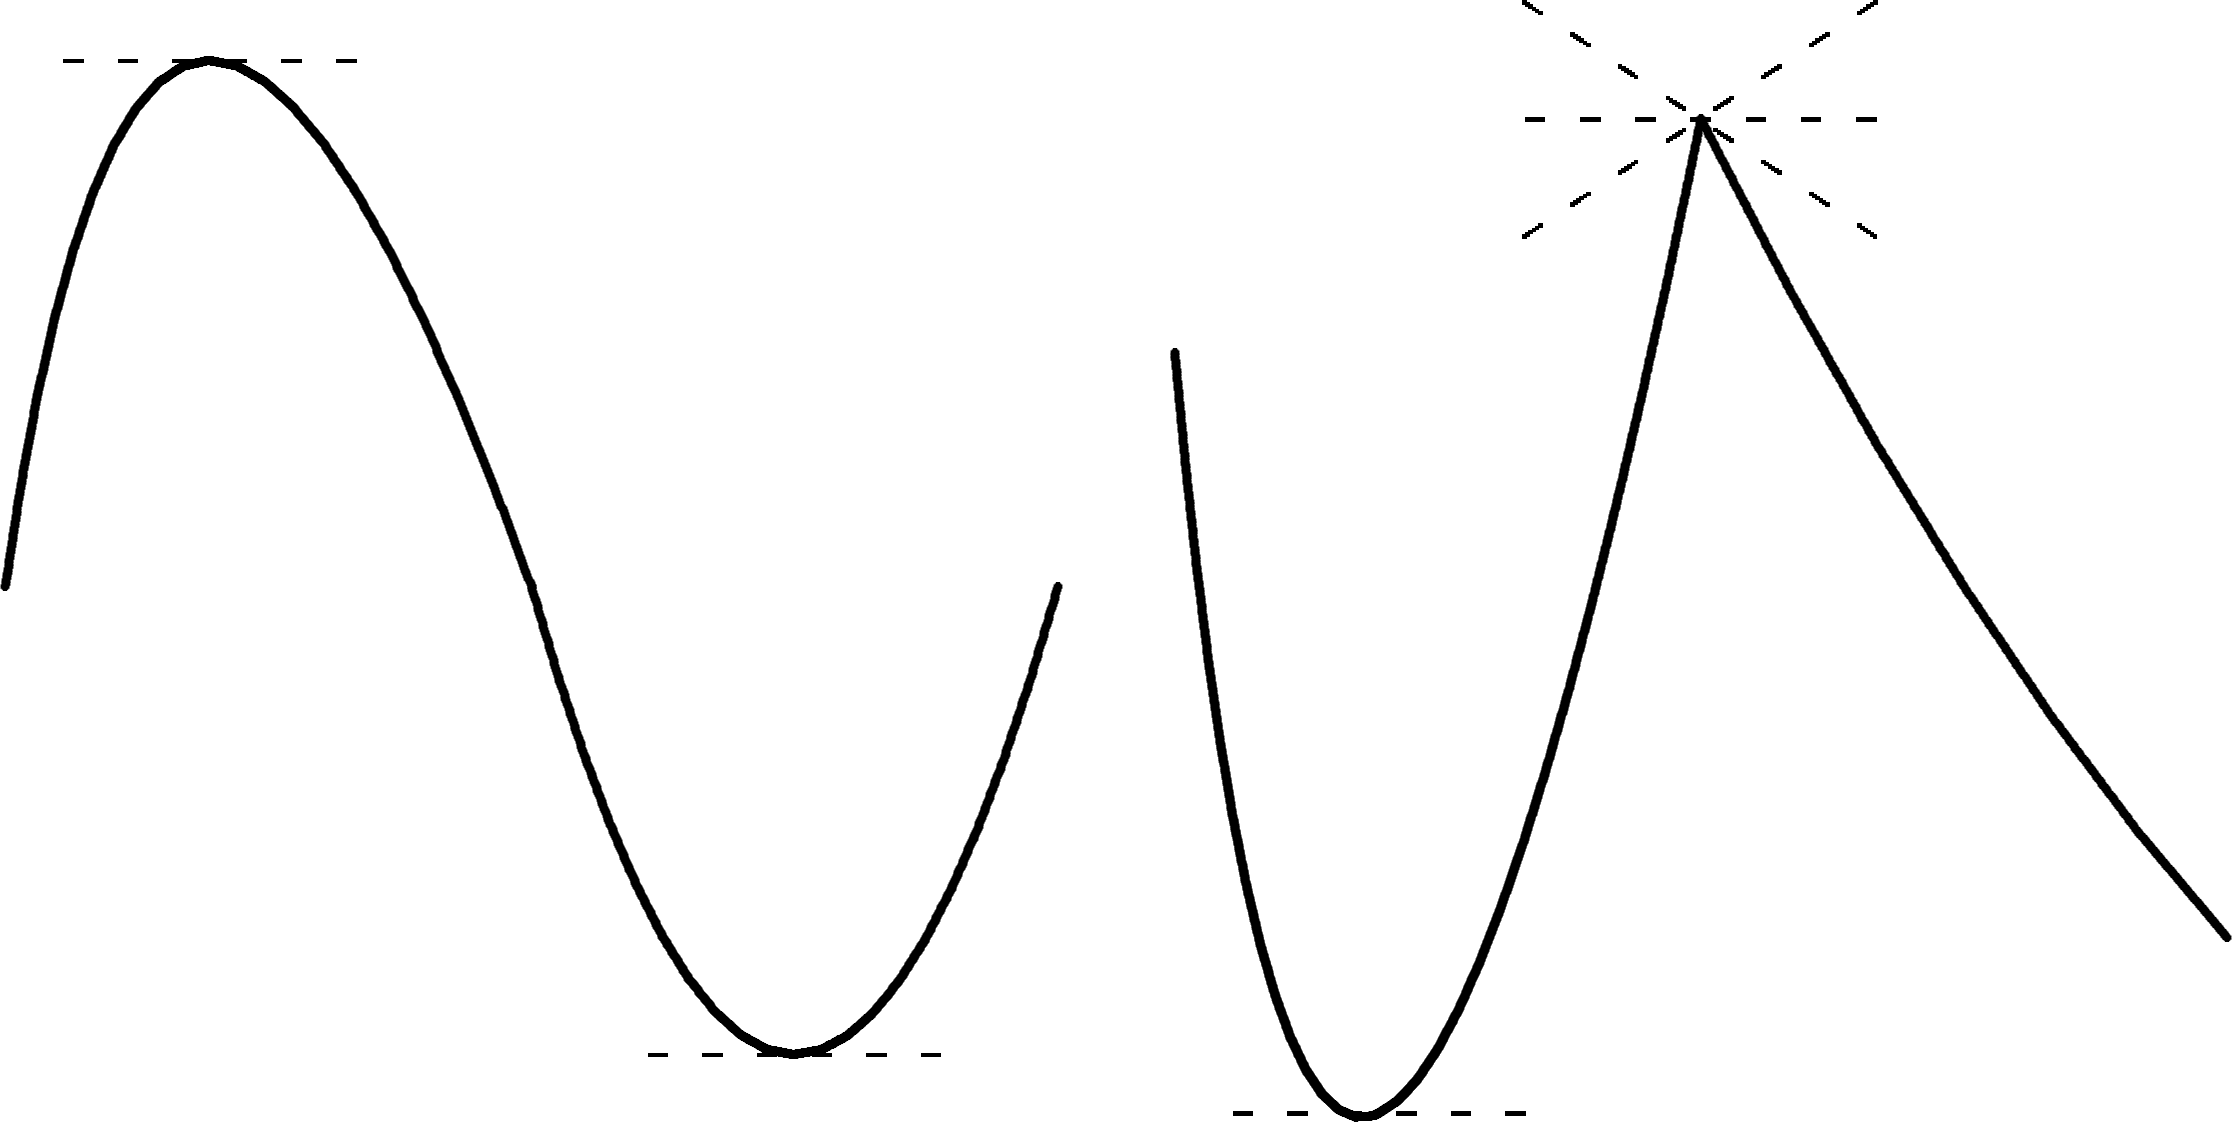
\includegraphics[width=0.6\textwidth]{Images/extrema.png}
\caption[\small Critical points for continuous functions of a real variable]{\small Critical points for continuous functions of a real variable.}\hrule\label{fig:extrema}
\end{figure*}
Optimisation is quite possibly the most-commonly used application of the derivative. You will recall that a differentiable function $f:[a,b]\to \mathbb{R}$ has a \textbf{critical point} at $x^*\in (a,b)$ if either $f(x^*)=0$ or $f'(x^*)$ is undefined (see Figure~\ref{fig:extrema}). If additionally $f$ is continuous, then the optimal solution of the problem
\[\begin{array}{rl}
\max & f(x) \\
\mbox{s.t.} & x\leq b \\ 
 & x\geq a \\ 
&x \in \mathbb{R}
\end{array}\]
is found at one (or possibly, many) of the following feasible solutions: $x=a$, $x=b$, or $x=x^*$ where $x^*$ is a critical point of $f$ in $(a,b)$.\newl This can be extended fairly easily to multi-dimensional domains, with the following theorem. 
\newl \textbf{Theorem} let $f:\mathcal{A}\subseteq \mathbb{R}^n\to \mathbb{R}$ be a continuous function, where $\mathcal{A}$ is a closed subset of $\mathbb{R}^n$. Then $f$ reaches its maximum (resp. minimum) value either at a critical point of $f$ in the interior of $\mathcal{A}$, or somewhere on $\partial\!\!\mathcal{A}$, the \textbf{boundary} of $\mathcal{A}$. 
\begin{center}\rule{0.5\linewidth}{.4pt}\end{center}
Consider, for instance, a company that sells gadgets and gizmos. Let's say that the company's monthly profits are expresses (in 1000\$s of dollars) according to $$f(x,y)=81+16xy-x^4-y^4, $$ where $x$ and $y$ represent, respectively, the number of gadgets and gizmos sold monthly (in 10,000s of units). What is the optimal number of each items that the company must sell in order to maximise its profits?\newl Since $f$ is continuous, the maximum value is reached at a critical value in $$\mathcal{A}^{\circ}=(0,3)\times (0,3)$$ or somewhere on the boundary $$\partial\!\!\mathcal{A}=\{(x,y)|x=0 \mbox{ or }x=3\mbox{ or }y=0\mbox{ or }y=3\}.$$
But $f$ is smooth; the gradient $\nabla f(x,y)$ is thus always defined, and the only critical points are those for which $\nabla f(x,y)=(16y-4x^3,16x-4y^3)=(0,0)$. At such a point, $4x=y^3$, which, upon substitution in $f_x$ yields $$0=16y-\frac{1}{16}y^9=\frac{1}{16}y(256-y^8)=\frac{1}{16}y(y-2)(y+2)(y^2+4)(y^4+16), $$ which is to say $y=-2,0,2$. Only $y=2$ can potentially yield a critical point in $\mathcal{A}^{\circ}$, however. When $y=2$, $x=\frac{1}{4}2^3=2$: the only critical point of $f$ in $\mathcal{A}^{\circ}$ is thus $(x^*,y^*)=(2,2)$, and the function value at that point is $$f(x^*,y^*)=81+16(2)(2)-2^4-2^4=113.$$  On the boundary $\partial\!\! \mathcal{A}$, the objective function reduces to one of the following four forms 
\begin{align*} 
f(0,y)=g_0(y)&=81-y^4,\quad \mbox{on }0\leq y\leq 3 \\ 
f(3,y)=g_3(y)&=48y-y^4, \quad \mbox{on }0\leq y\leq 3 \\ 
f(x,0)=h_0(x)&=81-x^4,\quad \mbox{on }0\leq x\leq 3  \\ 
f(x,3)=h_3(x)&=48x-x^4, \quad \mbox{on }0\leq x\leq 3 
\end{align*}
These functions are easy to optimise, being continuous functions of a single real variable; $g_0$ and $h_0$ are maximised at the origin, with the objective function taking the value 81 there, while $g_3$ and $h_3$ are maximised at $12^{1/3}$, with the objective function taking the value $\approx 82.42$ there. \newl Combining all this information, we conclude that the company will maximise its profits if it sells 20,000 units of both the gadgets and the gizmos.  
\begin{center}\rule{0.5\linewidth}{.4pt}\end{center}
While the approach we just presented works in this case, there are many instances for which it can be substantially more difficult to find the optimal value on $\partial\!\!\mathcal{A}$. The method of \textbf{Lagrange multipliers} can simplify the computations, to some extent. \newl Consider the problem
\[\begin{array}{rl}
\min/\max & f(\mathbf{x}) \\
\mbox{s.t.}
 & g_i(\mathbf{x})\leq a_i \quad i = 1,\ldots,m \\
 & \mathbf{x} \in \mathcal{D},
\end{array}\]
where $f$ and $g$ are continuous and differentiable on the (closed) region $\mathcal{A}$ described by the constraints $g_i\leq a_i$ (strictly speaking, differentiability is not required on all of $\mathcal{A}$). If the problem is feasible and bounded, then the optimal value is reached either at a critical point of $f$ in $\mathcal{A}^{\circ}$ or at a point $\mathbf{x}\in\partial\!\! \mathcal{A}$ for which $$\nabla f(\mathbf{x})=\lambda_1 \nabla g_1(\mathbf{x})+\cdots + \lambda_m\nabla g_m(\mathbf{x}),$$ where $\lambda_1,\ldots,\lambda_m\in \mathbb{R}$ are the Lagrange multipliers of the problem.   
\begin{center}\rule{0.5\linewidth}{.4pt}\end{center}
For instance, consider a factory that produces deluxe pickle jars. The monthly number of jars $Q$ that can be produced at the factory is given by 
$Q(K,L)=900K^{0.6}L^{0.4},$  where $K$ is the monthly available capital, and $L$ is the factory's workforce monthly pay. Each deluxe pickle jar requires $100\$$ in workforce pay, and $200\$$ in capital (the pickles are extra deluxe, apparently). If the factory owners want to maintain monthly production at 36,000, what combinations of capital and workforce pay will minimise the total production costs? \newl The optimisation problem is 
\[\begin{array}{rl}
\min & f(K,L)=200K+100L \\
\mbox{s.t.}
 & K^{0.6}L^{0.4}=40 \\ 
 & K,L \geq 0.
\end{array}\]
The objective function is linear and so has no critical point. The feasability region $\mathcal{A}$ can be described by the constraints $g_1(K,L)=K^{0.6}L^{0.4}\leq 40$ and $g_2(K,L)=-K^{0.6}L^{0.4}\leq -40$. Points of interest on the boundary $\partial\!\!\mathcal{A}$ are obtained by solving the Lagrange equation 
\begin{align*}(200,100)&=\lambda_1\left(0.6\left(\frac{L}{K}\right)^{0.4},0.4\left(\frac{K}{L}\right)^{0.6}\right)-\lambda_2\left(0.6\left(\frac{L}{K}\right)^{0.4},0.4\left(\frac{K}{L}\right)^{0.6}\right) \notag \\ &=\lambda\left(0.6\left(\frac{L}{K}\right)^{0.4},0.4\left(\frac{K}{L}\right)^{0.6}\right) \quad\mbox{since }\nabla g_1 = -\nabla g_2, \end{align*} with $K^{0.6}L^{0.4}=40.$ Numerically, there is only one solution, namely  $$(K_*,L_*,\lambda)\approx (35.65,47.54,297.10).$$ The objective function at that point takes on the value $$f(K_*,L_*)\approx 200(35.65)+100(47.54)\approx 11884.02,$$ and we know that this value must either be the maximum or the minimum of the objective function subject to the constraints of the problem. We know, however, that the point $(K_1,L_1)= (1,40^{2.5})$ belongs to $\partial\!\!\mathcal{A}$; since $$f(K_1,L_1)=200(1)+100(40^{2.5}) >  f(K_*,L_*),$$ then $(K_*,L_*)$ is indeed the minimal solution of the problem, and the minimal value of the objective function is $\approx 11,884.02\$$. 
\begin{center}\rule{0.5\linewidth}{.4pt}\end{center} Given how straightforward the method is, it might seem that there is no real need to say anything else -- why would anybody ever use something other than Lagrange multipliers to solve optimisation problems? One of the issues is that when the number of constraints is too high relative to the dimension of $\mathcal{D}$, which is usually the case in real-life situations, then there may not be a finite number of candidates solutions on $\partial \!\! \mathcal{A}$, which makes this approach useless. 
\section{Classification of Optimisation Problems and Types of Algorithms}
The computational difficulty of optimisation problems, then, depends on the
properties of the domain set, constraints, and the objective function.
\subsection{Classification} Problems without constraints are said to be \textbf{unconstrained}. For
example, least-squares minimisation in statistics can be formulated as
an unconstrained problem, and so can \[\begin{array}{rl}
\min & x^2 - 3x \\
\mbox{s.t.} & x \in \mathbb{R}
\end{array}\]
Problems with linear constraints $g_i$ (that is, linear inequalities or
equalities) and a linear objective function $f$ form an important class of
problems in \textbf{linear programming}. Linear programming problems are by far 
the \textbf{easiest} to solve in the sense that efficient algorithms exist
both in theory and in practice. Linear programming is also the backbone
for solving more complex models  \cite{OPT_BT}.
\newl
\textbf{Convex problems} are problems with a convex domain set -- a set $\mathcal{D}$ such that $$t\mathbf{x}_1+(1-t)\mathbf{x}_2\in \mathcal{D},\ \forall \mathbf{x}_1,\mathbf{x}_2\in \mathcal{D},\forall t\in [0,1],$$ convex
constraints $g_i$ and a convex objective function $f$ -- i.e.  $$h(t\mathbf{x}_1+(1-t)\mathbf{x}_2)\leq th(\mathbf{x}_1)+(1-t)h(\mathbf{x}_2),\ \forall \mathbf{x}_1,\mathbf{x}_2\in \mathcal{D},\forall t\in [0,1], h\in \{f,g_i\}.$$ Convex optimisation
problems have the property that \textbf{every local optimum is also a global
optimum}. Such a property permits the development of effective algorithms
that could also work well in practice. Linear programming is a special
case of convex optimisation.\newl \textbf{Nonconvex problems} (such as problems involving integer variables and/or nonlinear constraints that are not convex) are the hardest problems to
solve. In general, nonconvex problems are \textbf{NP-hard}. Such problems often arise in scheduling and engineering applications.
\newl In the rest of this section, we will primarily focus  on linear programming and nonconvex
problems whose linear constraints $g_i$ and objective function $f$ are linear, but with domain set $\mathcal{D}\subseteq \mathbb{R}^k \times \mathbb{Z}_+^{n-k}$. These
problems cover a large number of applications in operations research, 
which are often discrete in nature.
\newl We will not discuss optimisation problems that arise in statistical learning and engineering
applications that are modeled as nonconvex continuous models since they require different sets of techniques
and methods -- more information is available in \cite{OPT_B}.

\begin{center}\rule{0.5\linewidth}{.4pt}\end{center}

\subsection{Algorithms}
We will not go into the details of algorithms for solving the
problems discussed, as consultants are expected to be using \textbf{off-the-shelf}
solvers for the various tasks, but it could prove useful for the analyst to know the 
various types of algorithms or methods that exist for solving
optimisation problems.
\newl Algorithms fall into two families: \textbf{heuristics} and \textbf{exact} methods.\begin{itemize}[noitemsep]
\item Heuristics are normally quick to execute but do not provide guarantees
of optimality. For example, the greedy heuristic for the Knapsack
Problem is very quick but does not always return an optimal solution. In
fact, there is no guarantee on how good a solution is. Other heuristics
methods include \textbf{ant colony}, \textbf{particle swarm}, and \textbf{evolutionary algorithms},
just to name a few. There are also heuristics that are stochastic in
nature and have proof of convergence to an optimal solution. Simulated
annealing and multiple random starts are such heuristics. Unfortunately,
there is no guarantee on the running time to reach optimality and there
is no way to identify when one has reached an optimum.
\item Exact methods return a global optimum after finite time. However, most
exact methods only guarantee that constraints are approximately
satisfied though the violation is below some pre-specified tolerance. It
is therefore possible for the returned solutions to be infeasible for
the actual problem. There also exist exact methods that fully control
the error. When using such a method, an optimum is usually given as a
\textbf{box guaranteed to contain an optimal solution} rather than a single
element. Returning boxes rather than single elements are needed in
cases, for example, where the optimum cannot be expressed exactly as a
vector of floating point numbers. Such exact methods are used mostly in
academic research and in areas such as medicine and avionics where the
tolerance for errors is practically zero.
\end{itemize}

\section{Linear Programming}

Linear programming was initially developed independently by George B.
Dantzig and Leonid Kantorovich in the first half of the $20^{\textrm{th}}$ century to
solve resource planning problems. Even though linear programming is
insufficient for many modern-day applications in operations research, it
was useful in many economic and military contexts in the early days. To
motivate some key ideas in linear programming, we begin with a small
example.\begin{center}\rule{0.5\linewidth}{.4pt}\end{center} Say you are a vendor of lemonade and lemon juice. Each unit of lemonade
requires 1 lemon and 2 litres of water to prepare, and each unit of lemon juice
requires 3 lemons and 1 litre of water to prepare. Each unit of lemonade gives a
profit of 3\$ dollars upon selling, and each unit of lemon juice gives a profit of 2\$
dollars, upon selling. You have 6 lemons and 4 litres of water available. How many
units of lemonade and lemon juice should you prepare in order to maximise profit?
\par If we let \(x\) and $y$ denote the number of units of
lemonade and lemon juice, respectively, to prepare, then the profit is the objective function,  given by \(3x + 2y\) \$. Note that there are a number of
constraints that \(x\) and \(y\) must satisfy: 
\begin{itemize}[noitemsep]
\item \(x\) and \(y\) should be non-negative;
\item the number of lemons needed to make \(x\)
units of lemonade and \(y\) units of lemon juice is \(x+3y\) and cannot
exceed 6;
\item the number of litres of water needed to make \(x\) units of
lemonade and \(y\) units of lemon juice is \(2x+y\) and cannot exceed 4;
\end{itemize}
Hence, to determine the maximum profit, we need to maximise \(3x + 2y\)
subject to \(x\) and \(y\) satisfying the constraints \(x + 3y \leq 6\),
\(2x + y \leq 4\), \(x \geq 0\), and \(y \geq 0.\)
\newl A more compact way to write the problem is as follows:
\[\begin{array}{rrcrll}
\max & 3x & + & 2y & \\
\mbox{s.t.}
& x & + & 3y & \leq & 6 \\
& 2x & +&  y & \leq & 4 \\
& x &  & & \geq & 0 \\
& & & y & \geq & 0. \\
& x & , & y & \in & \mathbb{R}.
\end{array}\] It is customary to omit the specification of the domain
set in linear programming since the variables always take on real
numbers. Hence, we can simply write \[\begin{array}{rrcrll}
\max & 3x & + & 2y & \\
\mbox{s.t.}
& x & + & 3y & \leq & 6 \\
& 2x & +&  y & \leq & 4 \\
& x &  & & \geq & 0 \\
& & & y & \geq & 0.
\end{array}\]
\newl We can solve the above maximisation problem graphically, as follows. We
first sketch the set of \(\begin{bmatrix} x, y\end{bmatrix}^{\!\top}\)
satisfying the constraints, called the \textbf{feasible region}, on the
\((x,y)\)-plane. \par We then take the objective function \(3x+2y\) and turn
it into the equation of a line \(3x+2y = c\) where \(c\) is a parameter.
Note that as the value of \(c\) increases, the line defined by the
equation \(3x+2y=c\) moves in the direction of the normal vector
\(\begin{bmatrix} 3,2\end{bmatrix}^{\!\top}\). We call this direction the
\textbf{direction of improvement}. \par Determining the maximum value of the objective
function, called the optimal value, subject to the contraints amounts to
finding the maximum value of \(c\) so that the line defined by the
equation \(3x+2y=c\) still intersects the feasible region. \newl Figure~\ref{fig:lemon}
\begin{figure*}[!t]
\centering 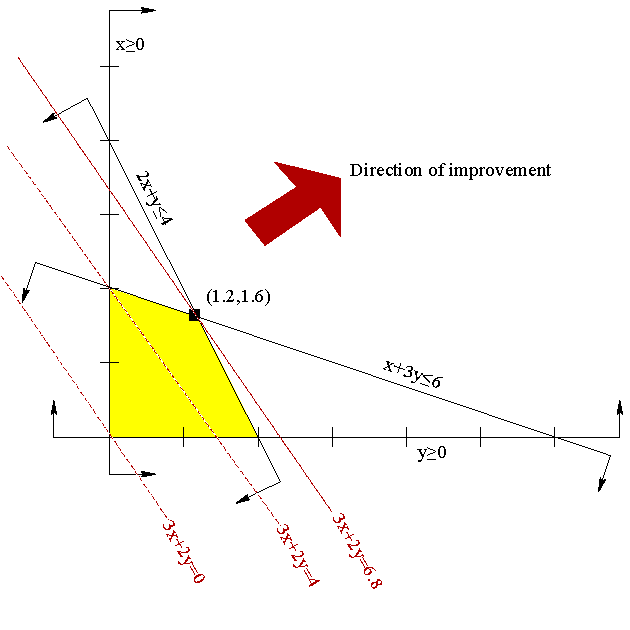
\includegraphics[width=0.7\linewidth]{Images/lemon} 
\caption[\small Graphical solution for the lemonade and lemon juice problem]{\small Graphical solution for the lemonade and lemon juice optimisation problem; the feasible region is shown in yellow, and level curves of the objective function in red. }\hrule \label{fig:lemon}
\end{figure*}
shows the lines with \(c=0,4,6.8\). We can see that
if \(c\) is greater than 6.8, the line defined by \(3x+2y = c\) will not
intersect the feasible region. Hence, the profit cannot exceed 6.8
dollars.

As the line \(3x+2y = 6.8\) does intersect the feasible region, \(6.8\)
is the maximum value for the objective function. Note that there is only
one point in the feasible region that intersects the line \(3x+2y=6.8\),
namely
\(\begin{bmatrix} x^*, y^*\end{bmatrix}^{\!\top} = \begin{bmatrix} 1.2, 1.6\end{bmatrix}^{\!\top}.\)
In other words, to maximise profit, we want to prepare 1.2 units of
lemonade and 1.6 units of lemon juice.
\newl This solution method can hardly be regarded as rigorous because we
relied on a picture to conclude that \(3x + 2y \leq 6.8\) for all
\(\begin{bmatrix} x,y\end{bmatrix}^{\!\top}\) satisfying the constraints.\newl But we
can actually obtain  this result \textbf{algebraically}. Note that multiplying both
sides of the constraint \(x + 3y \leq 6\) by \(0.2\) gives
\(0.2x + 0.6 y \leq 1.2\), and multiplying both sides of the constraint
\(2x + y \leq 4\) by \(1.4\) gives \(2.8x + 1.4 y \leq 5.6\). Hence, any
\(\begin{bmatrix} x,y\end{bmatrix}^{\!\top}\) that satisfies both \(x+3y\leq 6\)
and \(2x+y \leq 4\) must also satisfy
\((0.2x+0.6y) + (2.8x+1.4y) \leq 1.2 + 5.6\), which simplifies to
\(3x + 2y \leq 6.8\), as desired! 
\begin{center}\rule{0.5\linewidth}{.4pt}\end{center}
It is always possible to find an algebraic proof like the one above for
linear programming problems, which adds to their appeal. To describe the full result, it is
convenient to call on \textbf{duality}, a central notion in mathematical
optimisation.
\subsection{Linear Programming
Duality}
Let (P) denote following linear programming problem:
\[\begin{array}{rl}
\min & \mathbf{c}^\mathsf{T} \mathbf{x} \\
\mbox{s.t.} & \mathbf{A}\mathbf{x} \geq \mathbf{b}
\end{array}\] where \(\mathbf{c} \in \mathbb{R}^n\)
\(\mathbf{b} \in \mathbb{R}^m\)
\(\mathbf{A} \in \mathbb{R}^{m\times n}.\) (Here, inequality on tuples
is applied component-wise.) Then for every
\(\mathbf{y} \in \mathbb{R}^m_+\) (that is, all components of
\(\mathbf{y}\) are non-negative), the inferred inequality
\(\mathbf{y}^\mathsf{T}\mathbf{A}\mathbf{x} \geq \mathbf{y}^\mathsf{T} \mathbf{b}\)
is valid for all \(\mathbf{x}\) satisfying
\(\mathbf{A}\mathbf{x} \geq \mathbf{b}\). Furthermore, if
\(\mathbf{y}^\mathsf{T}\mathbf{A} = \mathbf{c}^\mathsf{T},\) the
inferred inequality becomes
\(\mathbf{c}^\mathsf{T} \mathbf{x} \geq  \mathbf{y}^\mathsf{T} \mathbf{b}\),
making \(\mathbf{y}^\mathsf{T} \mathbf{b}\) a lower bound on the optimal
value of (P). To obtain the largest possible bound, we can solve
\[\begin{array}{rl}
\max & \mathbf{y}^\mathsf{T} \mathbf{b} \\
\mbox{s.t.} & \mathbf{y}^\mathsf{T} \mathbf{A} = \mathbf{c}^\mathsf{T} \\
& \mathbf{y} \geq \mathbf{0}.
\end{array}\] This problem is called the \textbf{dual problem} of (P) and
(P) is called the \textbf{primal problem}.\newl A remarkable result relating
(P) and its dual (P') is the \textbf{Duality Theorem for Linear Programming}: if (P) has an optimal solution, then so does its dual 
problem (P'). Furthermore, the optimal values of the two problems are the
same.
\newl A \textbf{weaker result} follows easily from the discussion above: the objective function value of a feasible solution to
the dual problem (P') is a lower bound on the objective function value of a
feasible solution to (P).
\newl This result is known as \textbf{Weak Duality}. Despite the fact that it is a
simple result, its significance in practice cannot be overlooked because
it provides a way to gauge the quality of a feasible solution to (P). For example, suppose we have at hand a feasible solution to (P) with
objective function value 3 and a feasible solution to the dual problem (P') 
with objective function value 2. Then we know that the objective
function value of our current solution to (P) is within \(1.5\) times the
actual optimal value since the optimal value cannot be less than \(2\).
\newl In general, a linear programming problem can have a more complicated
form. Let \(\mathbf{A} \in \mathbb{R}^{m\times n}\),
\(\mathbf{b} \in \mathbb{R}^m\), \(\mathbf{c} \in \mathbb{R}^n\). Let
\({\mathbf{a}^{(i)}}^\mathsf{T}\) denote the \(i\)th row of
\(\mathbf{A}\), \(\mathbf{A}_j\) denote the \(j\)th column of
\(\mathbf{A}\), and (P) denote the minimisation problem, with variables in the tuple
\(\mathbf{x} = \begin{bmatrix} x_1, \cdots,  x_n\end{bmatrix}^{\!\top}\), given as follows
by:
\begin{itemize}[noitemsep]
\item
  the objective function to be minimised is
  \(\mathbf{c}^\mathsf{T} \mathbf{x}\);
\item
  the constraints are ${\mathbf{a}^{(i)}}^\mathsf{T}\mathbf{x}~\sqcup_i~b_i$, where \(\sqcup_i\) is \(\leq\), \(\geq\), or \(=\) for
  \(i = 1,\ldots, m\), and 
\item
  for each \(j \in \{1,\ldots,n\}\), \(x_j\) is constrained to be
  non-negative, nonpositive, or free (i.e.~not constrained to be
  non-negative or nonpositive.)
\end{itemize}
Then the \textbf{dual problem} (P') is defined to be the maximisation problem,
with variables in the tuple
\(\mathbf{y} = \begin{bmatrix} y_1, \cdots, y_m\end{bmatrix}^{\!\top}\) given
as follows:
\begin{itemize}[noitemsep]
\item
  the objective function to be maximised is
  \(\mathbf{y}^\mathsf{T} \mathbf{b}\);
\item
  for \(j = 1,\ldots, n\), the \(j\)th constraint is \begin{equation*}
  \left \{\begin{array}{ll}
  \mathbf{y}^\mathsf{T}\mathbf{A}_j \leq c_j & \text{if } x_j \text{ is
  constrained to be non-negative} \\
  \mathbf{y}^\mathsf{T}\mathbf{A}_j \geq c_j & \text{if } x_j \text{ is
  constrained to be nonpositive} \\
  \mathbf{y}^\mathsf{T}\mathbf{A}_j = c_j & \text{if } x_j \text{ is free}.
  \end{array}\right.
  \end{equation*}
\item
  and for each \(i \in \{1,\ldots,m\}\), \(y_i\) is constrained to be
  non-negative if \(\sqcup_i\) is \(\geq\); \(y_i\) is constrained to be
  nonpositive if \(\sqcup_i\) is \(\leq\); \(y_i\) is free if
  \(\sqcup_i\) is \(=\).
\end{itemize}
The following table can help remember the correspondences:
\begin{longtable}[]{@{}cc@{}}
\toprule
Primal (min) & Dual (max)\tabularnewline
\midrule
\endhead
\(\geq\) constraint & \(\geq 0\) variable\tabularnewline
\(\leq\) constraint & \(\leq 0\) variable\tabularnewline
\(=\) constraint & \(\text{free}\) variable\tabularnewline
\(\geq 0\) variable & \(\leq\) constraint\tabularnewline
\(\leq 0\) variable & \(\geq\) constraint\tabularnewline
\(\text{free}\) variable & \(=\) constraint\tabularnewline
\bottomrule
\end{longtable}
Below is an example of a primal-dual pair of problems based on the above
definition: Consider the primal problem: \[\begin{array}{rrcrcrcl}
\mbox{min} &  x_1 & - & 2x_2 & + & 3x_3 & \\
\mbox{s.t.} & -x_1 &   &      & + & 4x_3 &  =   &5 \\
            & 2x_1 & + & 3x_2 & - & 5x_3 & \geq &  6 \\
            &      &   & 7x_2 &   &      & \leq &  8 \\
            &  x_1 &   &      &   &      & \geq &  0 \\
            &     &    & x_2  &   &      & &      \mbox{free} \\
            &     &    &      &   & x_3  & \leq & 0.\\
\end{array}\]
Here,
\(\mathbf{A}= \begin{bmatrix}  -1 & 0 & 4 \\  2 & 3 & -5 \\  0 & 7 & 0 \end{bmatrix}\),
\(\mathbf{b} = \begin{bmatrix}5 \\6\\8\end{bmatrix}\), and
\(\mathbf{c} = \begin{bmatrix}1 \\-2\\3\end{bmatrix}\).
\newl 
The primal problem has three constraints. So the dual problem has three
variables. As the first constraint in the primal is an equation, the
corresponding variable in the dual is free. As the second constraint in
the primal is a \(\geq\)-inequality, the corresponding variable in the
dual is non-negative. As the third constraint in the primal is a
\(\leq\)-inequality, the corresponding variable in the dual is
nonpositive. Now, the primal problem has three variables. So the dual
problem has three constraints. As the first variable in the primal is
non-negative, the corresponding constraint in the dual is a
\(\leq\)-inequality. As the second variable in the primal is free, the
corresponding constraint in the dual is an equation. As the third
variable in the primal is nonpositive, the corresponding constraint in
the dual is a \(\geq\)-inequality. Hence, the dual problem is:
\[\begin{array}{rrcrcrcl}
\max & 5y_1 & + & 6y_2 & + & 8y_3 & \\
\mbox{s.t.} & -y_1 & + & 2y_2 &   &      & \leq &  1 \\
            &      &   & 3y_2 & + & 7y_3 & = & -2 \\
            & 4y_1 & - & 5y_2 &   &      & \geq &  3 \\
            &  y_1 &   &      &   &      &      &  \mbox{free} \\
            &     &    & y_2  &   &      & \geq & 0 \\
            &     &    &      &   & y_3  & \leq & 0.\\
\end{array}\]
In some books, the primal problem is always a \textbf{maximisation problem} -- in that case, what we have considered to be a primal problem is their dual problem and \textit{vice-versa}. Note that the \textbf{Duality Theorem for Linear Programming} remains true for the more general definition of the primal-dual pair of linear programming problems.

\subsection{Methods for Solving Linear Programming Problems}

There are currently two families of methods used by modern-day linear
programming solvers: \textbf{simplex methods} and \textbf{interior-point methods}. The
algorithms in either family are iterative. There is no known simplex
method that runs in polynomial time. In contrast, polynomial-time
interior-point methods that are also efficient in practice abound. We will not get into the technical details of these methods. \newl You might wonder why anyone would want to use simplex methods, even though they are not polynomial-time methods. Simplex methods are in general more \textbf{memory-efficient} than interior-point methods, and they tend to return solutions that have few nonzero entries. More
concretely, suppose that we want to solve the following:
\[\begin{array}{rl}
\min & \mathbf{c}^\mathsf{T}\mathbf{x} \\
\mbox{s.t.} & \mathbf{A}\mathbf{x} = \mathbf{b} \\
            & \mathbf{x} \geq \mathbf{0}.
\end{array}\] For ease of exposition, we assume that \(\mathbf{A}\) has
full row rank. Then, each iteration of a simplex method maintains a
current solution \(\mathbf{x}\) that is \textbf{basic}; that is, the columns of
\(\mathbf{A}\) corresponding to the nonzero entries of \(\mathbf{x}\)
are linearly independent. In contrast, interior-point methods will
maintain \(\mathbf{x} > \mathbf{0}\) throughout (whence the name
``interior point'').
\newl When one uses an off-the-shelf linear programming solver, the choice of
method is usually not too important since solvers have good defaults.
Simplex methods are typically used in settings when a problem needs to
be resolved after minor changes in the problem data or in problems with
additional integrality constraints discussed in the next section.


\section{Mixed-Integer Linear Programming
(MILP)}

For many real-life applications, the modeling power of linear
programming is insufficient. For example, there is no simple linear
programming formulation of the BKP. Fortunately,
allowing the domain set to restrict one or more variables to only
integer values drastically extends the modeling power. The price we pay
is that there is no guarantee that the problems can be solved in
polynomial time. We now consider an example.
\begin{center}\rule{0.5\linewidth}{.4pt}\end{center}
Recall the problem on lemonade and lemon juice mentioned earlier: the problem has a unique optimal solution at
\(\begin{bmatrix} x,y\end{bmatrix} = \begin{bmatrix} 1.2 , 1.6\end{bmatrix}^{\!\top}\)
for a profit of \(6.8\). But this solution requires us to prepare
\textbf{fractional units} of lemonade and lemon juice. What if we require the
number of units we prepare to be integers? We simply add integrality
constraints to the variables: \[\begin{array}{rrcrll}
\max & 3x & + & 2y & \\
\text{s.t.} 
& x & + & 3y & \leq & 6 \\
& 2x & +&  y & \leq & 4 \\
& x &  & & \geq & 0 \\
& & & y & \geq & 0 \\
& x &,& y & \in  & \mathbb{Z}. \\
\end{array}\] We no longer have a linear programming problem. Instead,
we have an \textbf{integer linear programming problem}. Note that we can solve
this problem via a case analysis. The second and third inequalities tell
us that the possible values for \(x\) are \(0\), \(1\), and \(2\). \begin{itemize}[noitemsep]
\item If
\(x = 0\), the first inequality gives \(3y \leq 6\), implying that
\(y \leq 2\). Since we are maximising \(3x+2y\), we want \(y\) to be as
large as possible. Note that
\(\begin{bmatrix} x,y \end{bmatrix}^{\!\top} = \begin{bmatrix} 0,2 \end{bmatrix}^{\!\top}\)
satisfies all the constraints with an objective function value of \(4\).
\item If \(x = 1\), the first inequality gives \(3y \leq 5\), implying that
\(y \leq 1\). Note that
\(\begin{bmatrix} x, y \end{bmatrix}^{\!\top} = \begin{bmatrix} 1, 1 \end{bmatrix}^{\!\top}\)
satisfies all the constraints with an objective function value of \(5\).
\item If \(x = 2\), the second inequality gives \(y \leq 0\). Note that
\(\begin{bmatrix} x, y \end{bmatrix}^{\!\top} = \begin{bmatrix} 2, 0 \end{bmatrix}^{\!\top}\)
satisfies all the constraints with an objective function value of \(6\).
\end{itemize}
Thus,
\(\begin{bmatrix} x^*,y^* \end{bmatrix}^{\!\top} = \begin{bmatrix} 2,0 \end{bmatrix}^{\!\top}\)
is an \textbf{optimal solution}.
\begin{center}\rule{0.5\linewidth}{.4pt}\end{center}
A \textbf{mixed-integer linear programming problem} (MILP) is a problem of
minimising or maximising a linear function subject to finitely many
linear constraints such that the number of variables are finite and at
least one of which is required to take on integer values.

If all the variables are required to take on integer values, the problem
is called a \textbf{pure integer linear programming problem} or simply an
\textbf{integer linear programming problem}. Normally, we assume the
problem data to be rational numbers to rule out pathological cases.
\newl Many solution methods for solving MILPs have been devised and some of
them first solve the \textbf{linear programming relaxation} of the
original problem, which is the problem obtained from the original
problem by dropping all the integrality requirements on the variables.
\newl For instance, if (MP) denotes the following mixed-integer linear programming problem:
\[\begin{array}{rrcrcrlll}
\min & x_1 &  &  & + & x_3  \\
\mbox{s.t.} & -x_1 & + &  x_2 & + &  x_3  & \geq & 1 \\
& -x_1 & - &  x_2 & + & 2x_3  & \geq & 0 \\
& -x_1 & + & 5x_2 & - &  x_3  & = & 3 \\
&  x_1 & , & x_2 & , & x_3 & \geq & 0 \\
&      &   &     &   & x_3  & \in & \mathbb{Z}. 
\end{array}\]
then the linear programming relaxation (P1) of (MP) is: \[\begin{array}{rrcrcrlll}
\mbox{min} & x_1 &  &  & + & x_3  \\
\text{s.t.} & -x_1 & + &  x_2 & + &  x_3  & \geq & 1 \\
& -x_1 & - &  x_2 & + & 2x_3  & \geq & 0 \\
& -x_1 & + & 5x_2 & - &  x_3  & = & 3 \\
&  x_1 & , & x_2 & , & x_3 & \geq & 0.
\end{array}\]
Observe that the optimal value of (P1) is a lower bound for the optimal value of (MP)
since the feasible region of (P1) contains all the feasible solutions to
(MP), thus making it possible to find a feasible solution to (P1) with
objective function value which is better than the optimal value of (MP). \par Hence,
if an optimal solution to the linear programming relaxation happens to
be a feasible solution to the original problem, then it is also an
optimal solution to the original problem. \par Otherwise, there is an integer
variable having a nonintegral value \(v\). What we then do is to create
two new sub-problems as follows: 
\begin{itemize}[noitemsep]
\item one requiring the variable to be at most the greatest integer less than \(v\), 
\item the other requiring the variable to be at least the smallest integer greater than \(v\).
\end{itemize}
This is the basic idea behind the \textbf{branch-and-bound method}. We now
illustrate these ideas on (MP).
\newl Solving the linear programming relaxation (P1), we find that
\(\mathbf{x}' = \frac{1}{3}\begin{bmatrix}0,2,1\end{bmatrix}^{\!\top}\)
is an optimal solution to (P1). Note that \(\mathbf{x}'\) is not a
feasible solution to (MP) because \(x'_3\) is not an integer. We now
create two sub-problems (P2) and (P3) such that (P2) is obtained from
(P1) by adding the constraint \(x_3 \leq \lfloor x'_3\rfloor\) and (P3)
is obtained from (P1) by adding the constraint
\(x_3 \geq \lceil x'_3\rceil\). (For a number \(a\),
\(\lfloor a \rfloor\) denotes the \textbf{floor of} \(a\) and
\(\lceil a \rceil\) denotes the \textbf{ceiling of} \(a\).) Hence,
(P2) is the problem \[\begin{array}{rrcrcrlll}
\min & x_1 &  &  & + & x_3  \\
\text{s.t.} & -x_1 & + &  x_2 & + &  x_3  & \geq & 1 \\
 & -x_1 & - &  x_2 & + & 2x_3  & \geq & 0 \\
 & -x_1 & + & 5x_2 & - &  x_3  & = & 3 \\
 &      &   &      &   &  x_3  & \leq & 0 \\
 &  x_1 & , & x_2 & , & x_3 & \geq & 0,
\end{array}\] and (P3) is the problem \[\begin{array}{rrcrcrlll}
\min & x_1 &  &  & + & x_3  \\
\text{s.t.} & -x_1 & + &  x_2 & + &  x_3  & \geq & 1 \\
 & -x_1 & - &  x_2 & + & 2x_3  & \geq & 0 \\
 & -x_1 & + & 5x_2 & - &  x_3  & = & 3 \\
 &      &   &      &   &  x_3  & \geq & 1 \\
 &  x_1 & , & x_2 & , & x_3 & \geq & 0.
\end{array}\] Note that any feasible solution to (MP) must be a feasible
solution to either (P2) or (P3). Using the help of a solver, one sees
that (P2) is infeasible. The problem (P3) has an optimal solution at
\(\mathbf{x}^* = \frac{1}{5}\begin{bmatrix}0,4,5\end{bmatrix}^{\!\top}\),
which is also feasible for (MP). Hence,
\(\mathbf{x}^*\) is an
optimal solution of (MP).
\begin{center}\rule{0.5\linewidth}{.4pt}\end{center}
There is often a choice on which variable to branch on and a choice on
which sub-problem to solve next. It turns out that such choices can have
an impact on the total computation time. However, there are no
hard-and-fast rules that work well all the time. This in area of ongoing
research.

\subsection{Cutting Planes}

Difficult MILP problems often cannot be solved by branch-and-bound
methods alone. A technique that is typically employed in solvers is to
add valid inequalities to strengthen the linear programming relaxation.
Such inequalities, known as \textbf{cutting planes}, are known to be
satisfied by all the feasible solutions to the original problem but not
by all the feasible solutions to the initial linear programming
relaxation. 
\begin{center}\rule{0.5\linewidth}{.4pt}\end{center}
To illustrate the ideas, consider the following example:
\[\begin{array}{rrcrlll}
\min & 3x & + & 2y \\
\text{s.t.} & 2x & + & y & \geq & 1 \\
 &  x & + & 2y & \geq & 4 \\
 &  x & , & y & \in & \mathbb{Z}.
\end{array}\] An optimal solution to the linear programming relaxation
is
\(\begin{bmatrix} x^+, y^+ \end{bmatrix}^{\!\top} = \frac{1}{3}\begin{bmatrix} -2,7 \end{bmatrix}^{\!\top}\).
Note that adding the inequalities \(2x + y \geq 1\) and
\(x + 2y \geq 4\) gives \(3x + 3y \geq 5\), or equivalently,
\(x + y \geq \frac{5}{3}\). But \(x+y\) is an integer for every feasible
solution \(\begin{bmatrix} x,y \end{bmatrix}^{\!\top}\). Thus,
\(x + y \geq 2\) is a valid inequality for the original problem, but is
violated by \(\begin{bmatrix} x^+, y^+ \end{bmatrix}^{\!\top}\).
Hence, \(x + y \geq 2\) is a cutting plane. Adding this to the linear
programming relaxation, we have \[\begin{array}{rrcrlll}
\min & 3x & + & 2y \\
\text{s.t.} & 2x & + & y & \geq & 1 \\
 &  x & + & 2y & \geq & 4 \\
 &  x & + & y & \geq & 2.
\end{array}\] which, upon solving, yields 
\(\begin{bmatrix} x^*,y^* \end{bmatrix}^{\!\top} = \begin{bmatrix} -1,3 \end{bmatrix}^{\!\top}\)
as an optimal solution. Since all the entries are integers, this is also
an optimal solution to the original problem. \newl
Note that we have been lucky in the sense that adding one cutting plane solved the problem. In
practice, one often needs to add numerous cutting planes and then continue
with branch-and-bound to solve nontrivial MILP problems. Many methods for generating cutting planes exist -- the problem of generating effective cutting planes efficiently is still an active area
of research \cite{OPT_C}.
\section{A Sample of Some Useful Modeling
Techniques}
We have so far discussed the kinds of optimisation problems that can be
solved and what is available for solving them. Practical success, however, depends upon the effective translation and formulation of a problem description into a mathematical
programming problem, which is often an art as it is a science. We will not be discussing formulation techniques in this module (see \cite{OPT_W} for details) -- rather, we will  highlight  a few techniques
that often arise in business applications, which our examples have not covered so far. 
\subsection{Activation}
Sometimes, one may want to set a binary variable \(y\) to 1 whenever some
other variable \(x\) is positive. Assuming that \(x\) is bounded above
by \(M\), the inequality \[x \leq My\] will model the condition. Note that if there is no valid upper bound on \(x\), the condition cannot be modelled using a linear constraint.

\subsection{Disjunction}

Sometimes, one wants \(\mathbf{x}\) to satisfy at least one of a list of
inequalities; that is,
\[{\mathbf{a}^{(1)}}^\mathsf{T}\mathbf{x} \geq b_1 
 \lor {\mathbf{a}^{(2)}}^\mathsf{T}\mathbf{x} \geq b_2 
      \lor \cdots 
 \lor {\mathbf{a}^{(k)}}^\mathsf{T}\mathbf{x} \geq b_k.\] To formulate
such a disjunction using linear constraints, we assume that, for \(i = 1,\ldots,k\), there is a lower bound \(M_i\) on
\({\mathbf{a}^i}^\mathsf{T}\mathbf{x}\) for all
\(\mathbf{x}\in \mathcal{D}\). Note that such bounds exist when
\(\mathcal{D}\) is a bounded set which is often the case in
applications. The disjunction can now be formulated as the following
system where \(y_i\) is a new 0-1 variable for \(i = 1,\ldots,k\):
\[\begin{array}{l}
 {\mathbf{a}^{(1)}}^\mathsf{T}\mathbf{x} \geq b_1 y_1 + M_1(1-y_1) \\
 {\mathbf{a}^{(2)}}^\mathsf{T}\mathbf{x} \geq b_2 y_2 + M_2(1-y_2) \\
  \vdots \\
 {\mathbf{a}^{(k)}}^\mathsf{T}\mathbf{x} \geq b_k y_k + M_k(1-y_k) \\
  y_1 + \cdots + y_k \geq 1.
\end{array}\] Note that
\({\mathbf{a}^i}^\mathsf{T}\mathbf{x} \geq b_i y_i + M_i(1-y_i)\)
reduces to \({\mathbf{a}^i}^\mathsf{T}\mathbf{x} \geq b_i\) when
\(y_i = 1\), and to \({\mathbf{a}^i}^\mathsf{T}\mathbf{x} \geq M_i\)
when \(y_i = 0\), which holds for all \(\mathbf{x} \in \mathcal{D}.\)
Therefore, \(y_i\) is an activation for the \(i^{\textrm{th}}\) constraint, and at least one is
activated because of the constraint \(y_1 + \cdots + y_k \geq 1\).

\subsection{Soft Constraint}

Sometimes, one is willing to pay a price for a constraint to be
violated. Such a constraint is called a \textbf{soft constraint}. There
are situations in which having soft constraints are advisable (e.g.~when
having an infeasible problem as a result of enforcing all the
constraints is not an option.) We illustrate the idea on a modified
BKP. As usual, there are \(n\) items and item \(i\)
has weight \(w_i\) and value \(v_i>0\) for \(i = 1,\ldots, n\). The
capacity of the knapsack is denoted by \(K\). Now, suppose that we prefer not to take more than \(N\)
items,  but that the \textbf{preference} is not an actual constraint. We assign a penalty for its violation and use the following formulation:
\[\begin{array}{rl}
\max & \sum\limits_{i = 1}^n v_i x_i - p y\\
\mbox{s.t.} & \sum\limits_{i = 1}^n w_i x_i \leq K \\
  & \sum\limits_{i = 1}^n x_i - y \leq N \\
  & x_i \in \{0,1\} \quad i = 1,\ldots, n \\
  & y \geq 0.
\end{array}\] Here, \(p\) is a non-negative number of our choosing. As we
are maximising $$\sum\limits_{i = 1}^n v_i x_i - p y,$$ \(y\) is pushed
towards 0 when \(p\) is relatively large. Therefore, the problem will be
biased towards solutions that try to violate
$x_1+\cdots+x_n \leq N$ as little as possible.\par  What value to
choose for \(p\) requires experimentation; the general rule is that if
violation is costly in practice, we should set \(p\) to a high value. Otherwise, set it to a
moderate value relative to the coefficients of the variables in the
objective function value. Note that when \(p\) is set to zero, the
constraint $x_1+\cdots+x_n \leq N$ has no effect
because \(y\) can take on any positive value without incurring a
penalty.


\section{Software Solvers}

A wide variety of solvers exist for all kinds of optimisation problems.
The \href{https://neos-server.org/neos/}{NEOS Server} is a free online
service that hosts many solvers and is a great resource for
experimenting with different solvers on small problems.

For large or computationally challenging problems, it is advisable to
use a solver installed on a dedicated private machine. Note that
Microsoft Excel and SAS include a very capable solver for various kinds
of optimisation problems (more on the former in the next section). They can often be sufficient for many
purposes. 

For bigger problems, commercial solvers can be useful:
\begin{itemize}[noitemsep]

\item
  \newhref{https://www.ibm.com/analytics/cplex-optimiser}{IBM ILOG Cplex}
\item
  \newhref{http://www.gurobi.com/}{Gurobi}
\item
  \newhref{http://www.fico.com/en/products/fico-xpress-optimisation}{FICO
  Xpress Optimisation}
\end{itemize}
There are popular open-source solvers as well:

\begin{itemize}[noitemsep]

\item
  \newhref{https://projects.coin-or.org/Cbc}{CBC}
\item
  \newhref{https://www.gnu.org/software/glpk/}{GLPK}
\item
  \newhref{http://scip.zib.de/}{SCIP} (requires a commercial licence for
  consulting work)
\item
  \newhref{http://www.juliaopt.org/}{JuliaOpt}
\end{itemize}
We mention in passing that learning how to use of any of these solvers
effectively requires a significant time investment. In addition, it is
common to build optimisation models using a modeling system such as
\newhref{https://www.gams.com/}{GAMS} and \newhref{https://lindo.com/}{LINDO},
or a modeling language such as \newhref{https://ampl.com/}{AMPL},
\newhref{http://zimpl.zib.de/}{ZIMPL}, or
\newhref{https://jump.readthedocs.io/en/latest/}{JuMP}.

\section{Data Envelopment Analysis}
\begin{wraptable}{R}{0.40\textwidth}
  \begin{center}
    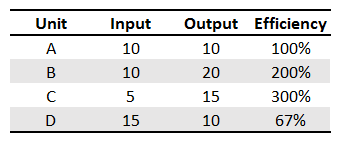
\includegraphics[width=0.4\textwidth]{Images/DEA1}
  \end{center}
  \caption{\small Simple input/output data for a fictional organisation.}\hrule
  \label{tab:DEA1}
\end{wraptable}
Operations Research (OR) is a mish-mash of various mathematical methods often used to solve complex industrial problems, especially optimisation problems, which are now being tackled in management and other non-industrial contexts. \textbf{Data envelopment analysis} (DEA), based on linear programming, is used to measure the relative performance of units in an organisation such as a government department, a school, a company, etc. \newl Typically, a unit's \textbf{efficiency} is defined as the quotient  of its outputs (activities of the organisation such as service levels or number of deliveries) by its inputs (the resources supporting the organisation's operations, such as wages or value of the in-store stock). In an organisation with only one type of input and one type of output, the comparison is simple (see for instance the data provided in Table~\ref{tab:DEA1}). 
However, if there are more than one input or output, the comparisons are less obvious: in Table~\ref{tab:DEA2}, is Unit $A$ more efficient than Unit $B$? Unit $A$ has fewer total inputs than Unit $B$ (as well as fewer outputs of type 1), but it has a substantially larger outputs of type 2. Without a system in place to measure the \textbf{relative efficiency}, comparison between (potentially incommensurable) units is unlikely to be fruitful. The relative efficiency of unit $k$ is defined by $$\mbox{RE}_k = \frac{\sum_j w_{k,j}O_{k,j}}{\sum_i v_{k,i}I_{k,i}}, $$ where $\{O_{k,j}|j=1,\ldots,n\}$ represent the $n$ outputs from unit $k$, $\{I_{k,i}|i=1,\ldots,m\}$ represent the $m$ inputs from unit $k$, and $\{w_{k,j}|j=1,\ldots,n\}$ and $\{v_{k,i}|i=1,\ldots, m\}$ are the \textbf{associated unit weights}. \newl For a specific unit $k$, the DEA model maximises the weighted sum of outputs for a fixed weighted sum of inputs (usually set to 100), subject to the weighted sum of outputs of every unit being at most equal to the weighted sum of its inputs when using the DEA weights of unit $k$ (in other word, the optimal set of weights for a given unit could not give another unit a relative efficiency greater than 1). This is equivalent to solving the following linear program for each unit $k_0$:   
  \begin{alignat*}{2}
    \text{max }   & \sum_{j=1}^n w_{k_0,j}O_{k_0,j} & &\  \\
    \text{s.t. } & \sum_{i=1}^m v_{k_0,i}I_{k_0,i} = 100 &\ & \\
                       & \sum_{j=1}^n w_{k_0,j}O_{\ell,j}-\sum_{i=1}^m v_{k_0,i}I_{\ell,i}\leq 0,\quad 1\leq \ell\leq K\\
                       & (w_{k_0,j},v_{k_0,i})\geq \mathbf{\varepsilon},\quad 1\leq j\leq n,\ 1\leq i\leq m &
  \end{alignat*}
  where $\varepsilon\geq 0$ is a parameter vector to be modified by the user. If we define $\mathbf{w}_{\ell}$,  $\mathbf{v}_{\ell}$, $\mathbf{O}_{\ell}$ and $\mathbf{I}_{\ell}$  as the vectors of output weights, input weights, outputs and inputs, respectively, for unit $\ell$, while $\mathbf{O}$ and $\mathbf{I}$ represent the row matrix of outputs and the row matrix of inputs for all the units, then the linear problem can be re-written simply as   
   \begin{alignat*}{2}
    \text{max }   & \mathbf{w}_{k_0}^{\!\top}\mathbf{O}_{k_0} \  \\
    \text{s.t. } & \mathbf{v}_{k_0}^{\!\top}\mathbf{I}_{k_0} = 100 ,\quad  \mathbf{w}_{k_0}^{\!\top}\mathbf{O}-\mathbf{v}_{k_0}^{\!\top}\mathbf{I}\leq \mathbf{0}, \quad -\left(\mathbf{w}_{k_0},\mathbf{v}_{k_0}\right)\leq -\mathbf{\varepsilon}  
  \end{alignat*} 
  This problem can be solved by the method of \textbf{Lagrange multipliers} or by using dedicated \textbf{numerical solvers}. \newl For the data 
\begin{table*}[t]
  \begin{center}
    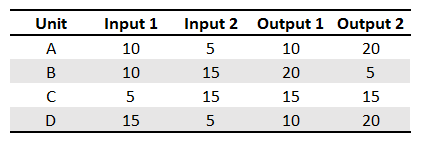
\includegraphics{Images/DEA2}
  \end{center}
  \caption{\small Double input/output data for a fictional organisation.}\hrule
  \label{tab:DEA2}
\end{table*}
  from Table~\ref{tab:DEA2}, the DEA program for unit $A$, for instance, becomes
  \begin{alignat*}{2}
    \text{max }   & 10w_{A,1}+20w_{A,2} \\
    \text{s.t. } & 10v_{A,1}+5v_{A,2} = 100 \\
                       & 10w_{A,1}+20w_{A,2}-10v_{A,1}-5w_{A,2}\leq 0 \\
                       & 20w_{A,1}+5w_{A,2}-10v_{A,1}-15w_{A,2}\leq 0 \\
                       & 15w_{A,1}+15w_{A,2}-5v_{A,1}-15w_{A,2}\leq 0 \\
                       & 10w_{A,1}+20w_{A,2}-15v_{A,1}-5w_{A,2}\leq 0 \\
                       & w_{A,1},w_{A,2},v_{A,1},v_{A,2}\geq \varepsilon
  \end{alignat*}

    \subparagraph*{Notes, Challenges and Pitfalls}
    \begin{itemize}[noitemsep]
    \item By allowing non-universal (unit-specific) weights, DEA allows each unit to present itself in the best possible light, which could potentially lead most units to be deemed efficient. This issue is mitigated when the number of units $K$ is greater than the product of the number of outputs by the number of inputs $n\cdot m$. 
    \item When the number of units is small, lack of differentiation among units is uninformative since all units could benefit from the best-case scenario described above. When there is differentiation, on the other hand, it can be quite telling: units with low DEA relative efficiency have achieved a low score \textit{even when given a chance to put their best foot forward}.   
\item Another concern is that a unit could artificially seem efficient by completely eliminating unfavourable outputs or inputs (i.e. if their associated weights are 0). Constraining the weights to take values in some fixed range can help avoid this issue. In the example that was discussed above, when we set $\varepsilon=0$, all units have a relative efficiency of 100. If we set $\varepsilon = 2$, however, the relative efficiencies are $\mbox{RE}_A=100$, $\mbox{RE}_B=67.7$, $\mbox{RE}_C=100$, and $\mbox{RE}_D=90$. Evidently, insisting that all the factors be considered changes the results.  
\item External factors can easily be added to the model as either inputs or outputs. Available resources are classified as inputs; activity levels or performance measures are classified as outputs. 
\item When units can also be assessed according to some other measure (such as profitability, average rate of success for a task, or environmental cleanliness, say), it can be tempting to use that other metric to rank the units. However, the combination of efficiency and profitability (or of any two measures, really) can offer insights and suggestions. \begin{description}
\item[Flagships] are units who score high on both measures and that can provide examples of good operating practices (as long as it is recognized that they are also likely beneficiaries of favorable conditions).  
\item[Sleepers] score low on efficiency but high on the other measure, which is probably more a consequence of favourable conditions than good management; as such, they become candidates for efficiency drives.  
\item[Dogs] score high on efficiency but low on the other measure, which indicates good management but unfavourable conditions. In extreme case, these units are candidates for closures, their staff members could be re-assigned to other units.  
\item[Question Marks] are units who score low on both measures; they are subject to unfavourable conditions, but this could also be a consequence of bad management. Attempts should be made to increase the efficiency of these units so that they become Sleepers or Flagships. 
\end{description}
\item The linear program to be solved (or its dual) gets complicated fairly quickly and  sophisticated software can be required to obtain a solution.  
\item \textbf{Advantages}: no need to explicitly specify a mathematical form for the production function; proven to be useful in uncovering relationships that remain hidden for other methodologies; capable of handling multiple inputs and outputs; capable of being used with any input-output measurement; the sources of inefficiency can be analysed and quantified for every evaluated unit.
\item \textbf{Disadvantages}: results are sensitive to the selection of inputs and outputs; cannot test for the best specification; the number of efficient units on the frontier tends to increase with the number of inputs and output variables.
    \end{itemize}
    \subsection{Excel and SAS Solvers}
As an illustration, consider the problem of finding the relative efficiency of unit $D$, in the example of the first section, that is, we are looking for the solution to 
  \begin{alignat*}{2}
    \text{max }   & 10w_{D,1}+20w_{D,2} \\
    \text{s.t. } & 15v_{D,1}+5v_{D,2} = 100 \\
                       & 10w_{D,1}+20w_{D,2}-10v_{D,1}-5w_{D,2}\leq 0 \\
                       & 20w_{D,1}+5w_{D,2}-10v_{D,1}-15w_{D,2}\leq 0 \\
                       & 15w_{D,1}+15w_{D,2}-5v_{D,1}-15w_{D,2}\leq 0 \\
                       & 10w_{D,1}+20w_{D,2}-15v_{D,1}-5w_{D,2}\leq 0 \\
                       & w_{D,1},w_{D,2},v_{D,1},v_{D,2}\geq 2
  \end{alignat*}
This is a small problem, and Excel's numerical solver can thankfully be used (see Table~\ref{tab:Excel}) to yield a relative efficiency of $90\%$. There are some issues with the solver, including the fact that a different worksheet has to be created for every single unit. There is presumably a way to set up the problem in order to compute the relative efficiency of all units simultaneously, but it's unlikely to be very flexible. With larger datasets, this approach may not be practical. 
\newl SAS's \texttt{proc optmodel}, available in versions 9.2 as part of the OR(R) suite can also be used; some work may have to be done to determine a way to automate the descriptions of the programs to be solved.    
\begin{table*}[t]
  \begin{center}
    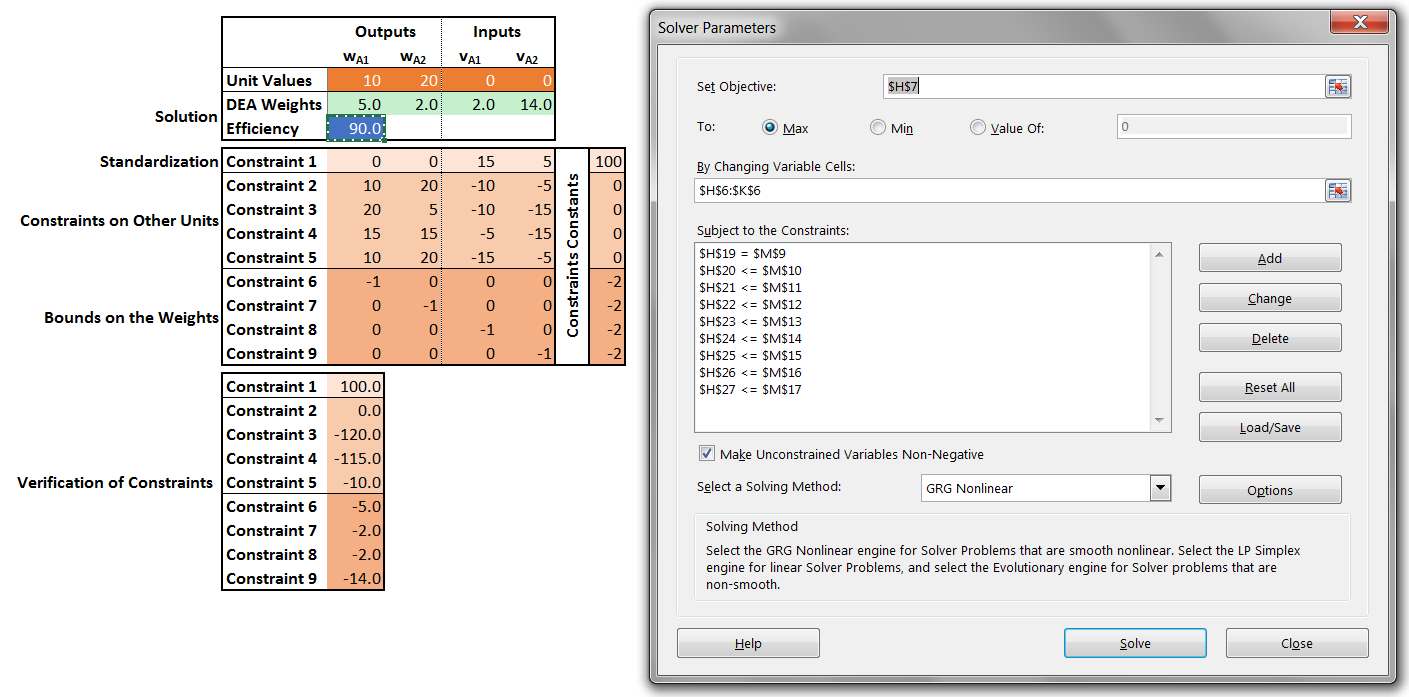
\includegraphics[width=\textwidth]{Images/DEA3}
  \end{center}
  \caption{\small Excel's numerical solver for unit $D$.}\hrule
  \label{tab:Excel}
\end{table*}
\section{Case Study: Resource Utilisation and Re-allocation in Barcelona Schools}
In this section, we present a illustration of a resource utlisation model which uses a DEA-like approach to illustrate that some flexibility is available.  
\begin{itemize}[noitemsep]
\item \textbf{Title:} On centralized resource utilisation and its re-allocation by using DEA
\item \textbf{Authors:} Cecilio Mar-Molinero,  Diego Prior, Maria-Manuela Segovia, Fabiola Portillo 
\item \textbf{Date:} 2012
\item \textbf{Methods:} Data envelopment analysis, simulations
\end{itemize}
\subsection*{Abstract} The standard DEA model allows different Decision-Making Unite (DMUs) to set their own priorities for the inputs and outputs that form part of the efficiency assessment. In the case of a centralized organisation with many outlets, such as an education authority that is responsible for many schools, it may be more sensible to operate in the most efficient way, but under a common set of priorities for all DMUs. The centralized resource allocation model does just this; the optimal resource reallocation is found for Spanish public schools and it is shown that the most desirable operating unit is a by-product of the estimation. 
\subsection*{Data}
The data consists of 54 secondary public schools in Barcelona during the year 2008, each with three discretionary inputs (teaching hours per week, $x_1$; specialized teaching hours per week, $x_2$; capital investments in the last decade, $x_3$), one non-discretionary input (total number of students present at the beginning of the academic year, $X$) and two outputs (number of students passing their final assessment, $y_1$, and number of students continuing their studies at the end of the academic year, $y_2$). A subset of the data is shown in Table~\ref{tab:spain}.
\begin{table*}[t]
  \begin{center}
    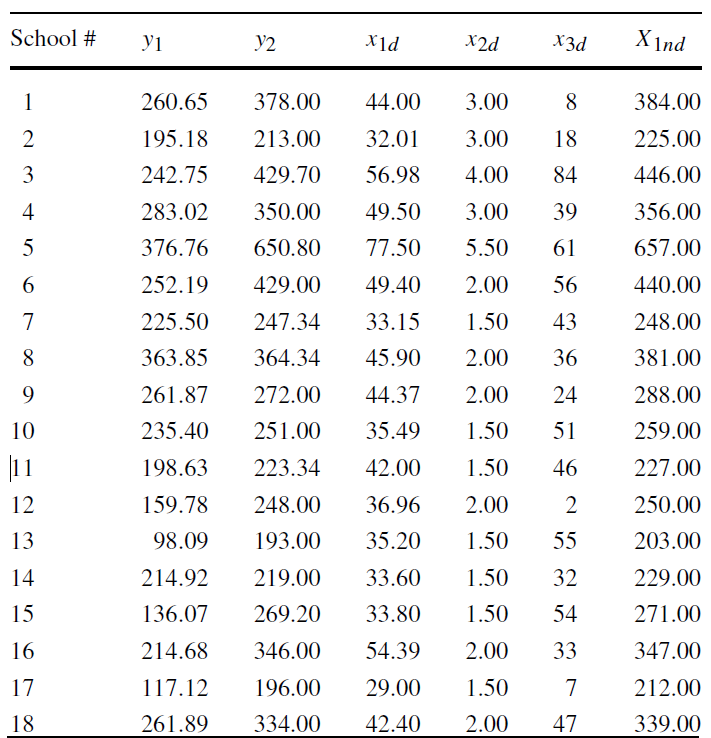
\includegraphics[width=0.58\textwidth]{Images/publicschooldata}
  \end{center}
  \caption[\small Sample from the Barcelona public school data.]{\small Sample from the Barcelona public school data set used to with the radial and simplified models.}\hrule
  \label{tab:spain}
\end{table*}
\subsection*{Challenges and Pitfalls}
\begin{itemize}[noitemsep]
\item The machinery of DEA cannot be brought to bear directly since the models under consideration are at best DEA-like.
\item The number of unknowns to be estimated in the original model is quadratic in the number of units. Consequently, the original model must be simplified to avoid difficulties when the number of units is large. Fortunately, the proposed simplifications can be interpreted logically in the context of re-allocation of resources.
\item There are situations where a solution to the simplified problem can be obtained even when the constraints on the total number of units is relaxed, allowing for the possibility of reaching the similar output levels with fewer inputs, in effect advocating for the closure of some units, but there are limitations: experiments show that this cannot be achieved with fewer than 32 schools (or with more than 81 schools).  
\end{itemize}
\subsection*{Project Summary and Results} In the standard DEA model, each unit sets its own priorities, and is evaluated using unit-specific weights. In a de-centralized environment, the standard approach is reasonable, but under a central authority where a common set of priorities needs to be met by all units (such as the branches of a bank, or recycling collection vehicles in a city), that approach needs to be modified. In a school setting, school board administrators may wish to evaluate teachers in a similar manner independently of the school at which they work.
\newl Centralized assessment imposes a common set of weights. For weakly centralized management, it is a further assumption that any input excess of inefficient units can be re-allocated among the efficient units, but only as long as this does not contravene the built-in inflexibilities of the system, which may make re-allocation rather difficult. Strongly centralized management, on the other hand, allow for re-allocation of the majority of inputs and outputs among all the units (inefficient or efficient) with the aim  of optimizing the performance of the entire system.\newl 
The original \textit{radial} model of Lozano and Villa is not, strictly speaking, a data envelopment model:
  \begin{alignat*}{2}
    \text{min }   & \theta & &\  \\
    \text{s.t. } & \sum_{r=1}^{54}\sum_{j=1}^{54} \lambda_{j,r}x_{i,j}-\theta \sum_{j=1}^{54}x_{i,j} \leq 0,  \quad\text{for }i=1,2,3 & \text{ (discretionary inputs)}& \\
    & \sum_{r=1}^{54}\sum_{j=1}^{54} \lambda_{j,r}X_{j}- \sum_{j=1}^{54}X_j \leq 0  &\text{ (non-discretionary input)} & \\
                       & \sum_{r=1}^{54}y_{kr}-\sum_{r=1}^{54}\sum_{j=1}^{54} \lambda_{j,r}y_{k,j}\leq 0, \quad \text{for }k=1,2 & \text{(outputs)}\\
                       & \sum_{j=1}^{54}\lambda_{j,r}=54,\quad \text{for }r=1,\ldots,54 &  &\\
                       & -\lambda_{j,r}\leq 0, \quad\text{ for }j,r=1,\ldots,54, \quad \theta \text{ free} & & 
  \end{alignat*}
Indeed, this model is not asking every unit to select the weights that make it look as good as possible when comparing itself to the remaining units under the same assessment: rather, the model is asking for the system as a whole to find the weights that present it in the best possible light possible, then it assesses the performance of the units separately, using the optimal system weights. \newl The main drawback of the radial model is the large number of weights to estimate. A simplification is proposed: if some of the units can be cloned, or equivalently, if some of the units can be closed and their resources re-allocated to other units, then the radial model becomes substantially simpler, and the number of weights to estimate is linear in the number of units (as opposed to quadratic).\newl The new
\begin{figure*}{t}
  \begin{center}
    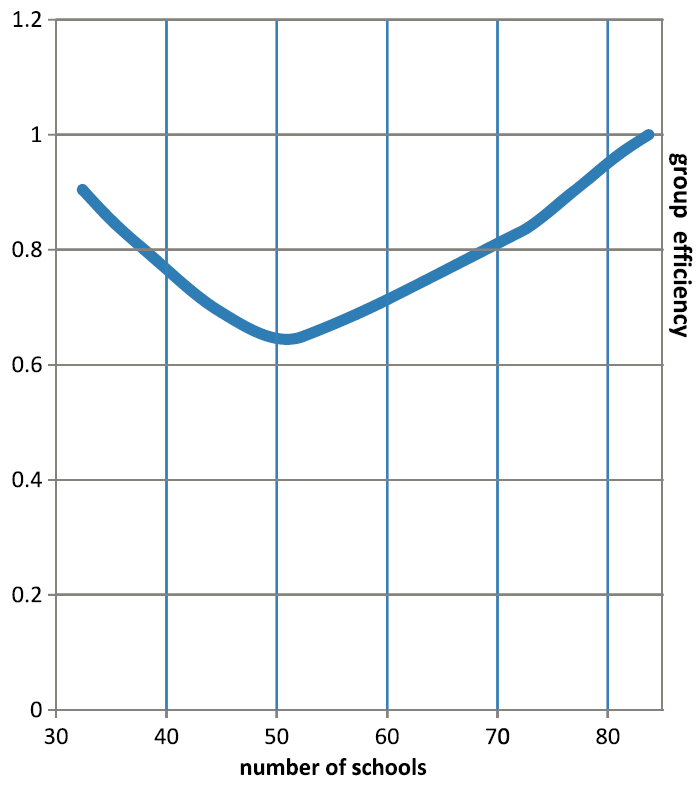
\includegraphics[width=0.3\textwidth]{Images/optimalefficiency}
  \end{center}
  \caption{\small Results of the re-allocation process in the Barcelona public school dataset.}\hrule
  \label{fig:overall}
\end{figure*}
 problem is DEA-like:
\begin{alignat*}{2}
    \text{min }   & \theta & &\  \\
    \text{s.t. } & \sum_{j=1}^{54} \lambda_{j}x_{i,j}-\theta \sum_{j=1}^{54}x_{i,j} \leq 0,  \quad\text{for }i=1,2,3 & \text{ (discretionary inputs)}& \\
    & \sum_{j=1}^{54} \lambda_{j}X_{j}- \sum_{j=1}^{54}X_j \leq 0  &\text{ (non-discretionary input)} & \\
                       & \sum_{r=1}^{54}y_{k}-\sum_{j=1}^{54} \lambda_{j}y_{k,j}\leq 0, \quad \text{for }k=1,2 & \text{(outputs)}\\
                       & \sum_{j=1}^{54}\lambda_{j}=54 &  &\\
                       & -\lambda_{j}\leq 0, \quad\text{ for }j=1,\ldots,54, \quad \theta \text{ free} & & 
  \end{alignat*}
The numerical solution to the radial model shows a group efficiency of 66\%, meaning that the outputs of the system could be produced while reducing the discretionary inputs by $\theta=34\%$. The simplified model reaches the same group efficiency by cloning units 25 (24.26 times), 26 (20.02 times), 36 (4.71 times), 17 (2.69 times), and 44 (1.70 times). The re-allocation of inputs and outputs among the 54 schools would produce the aforementioned reduction of the 34\% in discretionary inputs.\par 
A simulation experiment shows the effect of dropping the constraint on the number of units: the group efficiency obtained by solving the simplified system for various values of $n$ from 32 to 81 is seen in Figure~\ref{fig:overall}. Sure enough, the original solution is good, appearing near the minimum, which reaches $\theta=0.64$ at $n = 50.36$. This group efficiency corresponds to cloning units 25 (23.96 times), 26 (17.62 times), and 29 (7.87 times), Obviously, schools (and their resources) cannot be cloned, so what are we to make of this result?  It could be argued that unit 25 and 26, for instance, are ideal schools under the common priorities imposed by the system: should new schools have to be built, attempts could be made to emulate the stars.

\section{Case Study: Security Officer Profiles}
At airfields across the country, \textit{Borealian Airship Safety Authority}'s (BASA) security screening of passengers and their belongings is conducted
by \textbf{screening officers} (SO). The threat detection ability of a checkpoint is partially dependent on the skills of the SOs that operate it.
\par Consequently, BASA and its Screening Contractors must continuously train (and maintain) SOs to a
high level of security screening proficiency. This training includes `foundational' training and ongoing
training, such as \textit{recurrent learning} and $\gamma-$\textit{ray training} ($\gamma$RT) programs. System and SO performance are assessed through \textit{routine covert tests}, \textit{competency assessment sessions} and through the use of a \textit{threat-image projection system} (TIPS). Training and assessment serves a dual purpose: to maintain and improve the threat detection abilities of the screening workforce while also assessing individual SO performance.
\par To confirm that SOs continue to meet the certification standard, BASA is preparing to conduct
a certification maintenance review involving all 12,000+ SOs nationwide. Resources are limited and
assessment cannot be conducted personally for all SOs; as such BASA is seeking an approach which
would allow to target the certification maintenance towards SOs who work primarily in pre-board
screening (PBS) and who have demonstrated a lower propensity for detecting potential threats.
\par Given the varying types and quantities of data generated for each SO from their mandatory training
and assessment results, BASA wishes to have an \textbf{SO Indexing Tool} developed to support the SO
certification maintenance program.
%\subsection{Project Objective} The main objectives of the project are the following:
%\begin{itemize}[noitemsep]
%\item \textit{review BASA data}, particularly SO-specific data, to facilitate development of the Tool;
%\item \textit{conduct a literature review} to determine potential technique which could be used for the Tool;
%\item \textit{develop the Tool}, informed by the literature review using software and applications currently deployed at BASA (e.g. SAS, R, SPSS, Excel);
%\item \textit{develop a user guide} for the Tool;
%\item \textit{provide one-time training} on the Tool's functionality and usability, and 
%\item \textit{support initial implementation} of the Tool.
%\end{itemize}
\subsection{Project Scope and Considerations}
In a preliminary stage, BASA has selected \textbf{data envelopment analysis} (DEA) as the technique with which the Indexing Tool is to be developed. The main difficulties in that case remains to determine
\begin{itemize}[noitemsep]
\item which variables are \textbf{inputs}, and which are \textbf{outputs};
\item which ones are \textbf{discretionary} and which ones are \textbf{necessary};
\item what the lower bounds on the weights should be, and 
\item whether we want to present the system in the best light and find out which units best represent it, or whether we are looking to present each unit in the best light and care little for the system as a whole.
\end{itemize}
These are not trivial questions to answer. 
\subsection{Data}
BASA data comes in various flavours. Some of the data elements that may be used by the Tool for PBS are outlined below:
\begin{itemize}[noitemsep]
\item \textbf{Verification Testing (VT) Data:} covert tests are performed monthly at PBS checkpoints of Class A airfields -- all Class A sites conduct roughly the same number of tests each month; SOs at smaller airfields are re-tested more frequently and tend to have higher pass rates compared to SOs at larger airfields;
\item \textbf{Competency Session (CS) Data:} off-line timed tests conducted at Class A airfields. The number of monthly CS assessments conducted at a site is roughly proportional to the airfield's SO workforce;
\item \textbf{Threat-Image Projection System (TIPS) Data:} SO-specific $\gamma$-ray machine-based test. TIPS records the decision made by the SO at the X-ray station, the decision time, the type of threat projected, date/time/location of TIP events, and non-TIP false alarm counts;
\item \textbf{Advanced Threat Identification $\gamma-$ray (aTiX) Data:} since June 2X15, aTiX scanners run software which assist the SOs with detection of liquids and explosives. These units record data from each scanned item (e.g. scan timestamp, potential threat messages, operator decision) and the data is SO-specific (i.e., machines require SO login/logout). Processing rate, decision times and decision time-out frequencies can be derived from the available data; 
\item \textbf{$gamma-$ray Tutor ($\gamma$RT) Training Data:} mandatory lab-based educational program to which all SOs must dedicate a portion of their time. Data includes level-specific results (e.g. \% pass on various threat types, like Improvised Explosive Devices (IED)), and start and end dates, total time, and number of images viewed at each level.
\item \textbf{Performance-Related (Breach) Events (PE) Data:} breach- and SO-specific data available through the Learning Management System (LMS) database. May warrant consideration and or inclusion into the Tool.
\item \textbf{Recurrent Learning Program (RLP) Data:} results from the knowledge exam following basic screening training. May warrant consideration and inclusion into the Tool.
\item \textbf{Additional Assessment Data:} additional SO-specific data may become available in the future (such as a new mandatory national $\gamma-$ray exam to begin in 2X16). The Tool should allow for the inclusion of new variables. \end{itemize} Other factors to consider include the number of hours and passengers processed by SOs, the salaries (?), the fact that certain SOs have been tested substantially more often than other SOs; that the tool should be flexible to the number of variables to consider, and the number and class of SOs to include, and finally that an SOs total time of service should have a role to play in the index's determination. 
\newl One of the challenges facing policy makers in their decision process is that not every single SO has been tested to the same extent. Furthermore, those SOs who have been tested are by necessity only tested a small number of times, and as such their success rate may not be representative of their SO skills. Consequently, any DEA approach used in this context will need to incorporate features dealing with missing values, and uncertainty in some of the features. \newl Preliminary review suggests that missing values can be dealt with in one of three ways: \begin{itemize}[noitemsep]
\item by splitting the SOs according to which tests they have undertaken and running DEA models separately on each group; 
\item by comparing each unit to all units who have undertaken the same tests (and possibly more, but without involving the supplemental information), or 
\item by using an interval modifications. 
\end{itemize}
Similarly, a literature review suggests that uncertainty can be tackled using modified accuracy formulas, or discrete methods.
\subsection{Inputs, Outputs, Identifiers, Auxiliary Variables}
Upon discussion with BASA stakeholders and SMEs, a list of potential input and output variables for the DEA model was established. 
\newl The basic assumptions are that output measures should reflect \textbf{real-world security effectiveness and efficiency} (or situations taking place on the front lines, so to speak), whereas input measures should reflect any \textbf{resource expenditures that are undertaken to improve security effectiveness and efficiency}. 
\begin{itemize}[noitemsep]
\item\textbf{Identifiers:} LMS ID, airfield, Region, (airfield class), Length of employment (LMS), Average hours worked per active day (aTiX), Proportion of number of active days in the period of interest (or since employment began)* (SITT). 
\item\textbf{Filters:} $\gamma$RT data, TIPS data, RLP data must all be non-empty.
\item\textbf{Auxiliary Variables (for output adjustements):} VT count, TIPS count, Breach count (PEs), CS count.
\item\textbf{Inputs:} Highest level obtained, Overall success rate at last completed attempt ($\gamma$RT);
Total bags screened, Avg. number of bags screened per hour (aTiX); Total hours worked (PBS); Highest RLP exam score (LMS).
\item\textbf{Outputs (prior to adjustments):} \% Pass rate (VT); \% Pass rate, \% 'False Negatives rate (TIPS); Breach score (derived rate from breaches and total bag screens -- PEs, TIPS); \% Pass rate (CS).
\end{itemize}
It was ultimately decided that the RLP exam score should be removed from the list of inputs. Understandably, some fine-tuning will be required to determine any and all constraints on the weights (including removing a variable, or using linear combinations of variables): the nature of the data will determine the exact form of the DEA programs to solve for each airfield, region, or nationally.   
\subsection{Small Sample Sizes and Missing Data}
Only a fraction of SOs have data on all the measures. If the situation was that all of the selected input and output measures had data, then running DEA for different groupings of SOs (e.g. airfield, regional or national) would be straightforward.  However, having variables that have nulls for some SOs and not others presents a problem.  

One solution could be to cluster SOs into `data availability' groups and run separate DEAs for each group.  The problem here is that we would get DEA rankings that are not necessarily compatible from one cluster to another (an 85 in one group could mean anything from 0 to 100 in another group, for instance). Furthermore, the groups will  contain a smallish number of SOs; the DEA rankings within a group might not be able to do provide much in the way of differentiation. This is a big enough problem to warrant looking at alternatives which, while still not perfect, have fewer drawbacks. 
\newl Another solution is to collapse groups in a top-down manner: SOs with no missing variable only get compared to other SOs with no missing variable, but SOs with 1 specific missing variable get compared to all SOs with that 1 specific missing variable AND all SOs with no missing variable (for whom we drop the specific variable). There are a few problems with this approach: chiefly, not every unit is compared to every other unit, so that units with many tests may find themselves at a disadvantage (or at an advantage, it is hard to tell before running the DEA programs).  

Yet another solution may to be drop variables that have no data points.  For example, roughly 50\% of SOs had no VTs in the given data set.  Dropping that variable may allow for the use of a single DEA model that could cover all SO groupings.  The problem with this approach is that valuable SO-specific information would be dropped -- in this case, VT results.
\newl Linked to the issue of \textbf{data availability} is the issue of \textbf{data accuracy}: test results are used as proxy for SOs true abilities, but the sample sizes are (out of necessity) quite small. We can view missing data essentially as a sample of size 0. We would not trust a test result of 100\% to represent the true ability of the SO if only one test was given; rather, we should look for the expected value of the true ability, given the test results obtained so far, AND given the passing rate for the test in the SOs cohort. This correction allows us to dull the effects caused by small sample size, and to handle samples of size 0 with the same approach -- having no test score does not mean that we have NO information about the projected score based on other factors. Imputation by the corrected mean is suggested as a sound alternative to grouping SOs on the basis of their data availability: $$E\left(\text{test score}|n \text{ successes in }m \text{ trials}\right)=\frac{n+k}{m+k+1}, $$ where the specific value of $k$ is depends on the expected success rate of the SOs entire cohort. 

A general regression model to impute likely values for an SO score relative to its cohort (e.g. based on their location, experience, etc.) could also be used, and corrected as above, to represent the best guess of what the SOs actual score could be had the SO performed a sufficient number of tests.  
\par Multiple imputation could also be considered, if the tool's running time permits it -- we compute DEA scores for each iteration of the imputed dataset, and combine the DEA rankings to produce a final DEA ranking. The imputed values may or may not add much to the overall DEA ranking of an SO (i.e. a corrected mean value may water down a SOs efficiency ranking, or it could substantially modify it); ideally, imputed values would play a role analogous to that of a place holder -- they make it possible to run a single family of DEA programmes on the entire (applicable) SO population. However, since imputed values can potentially affect the overall ranking of the SOs, instances where imputed values are used by a DEA model should be flagged to allow for an assessment of the weight assigned to the imputed measure by the model.  If only a small number of SO DEA scores rely too heavily on the imputed measures, those SOs would be taken aside for further investigation. This would help ensure that imputed measures do not overly direct the outcome of the model. \par The final decision on this should, of course, be driven by the data: if this approach does not yield acceptable results, we may have no better option than to separate SOs into groups based on data availability and run separate DEA programs on these groups, with the caveats mentioned above.
%\subsection{Re-scaling Prior to Solving the DEA Problem}
%Finally, in order to be able to make inferences using the weight values, it will be expedient to re-scale each of the variables along interval $[0,1]$, where 1 corresponds to the maximum value of each variable within its group, while 0 still represents the smallest ``physical'' value that it can take: $y=x/x_{\text{max}}.$\newl At its most fundamental level, DEA deals with linear combinations of variables. Some non-linearity can be added to the picture simply by transforming the variables (this could prove useful, say, for variables for which a linear increase in level does not necessarily correspond to a linear increase in real performance): for instance, once $y$ is scaled along the interval $[0,1]$, the transformation $z=y^m$ has the effect of separating the best performances while clustering the poorer performances when $m>1$, and vice-versa when $m<1$.   
\subsection{DEA Model}
Ultimately, 5 inputs and 5 outputs were suggested:
\begin{description}[noitemsep]
\item[Inputs] $i_1$ -- average $\gamma$RT, in minutes spent per level; $i_2$ -- reversed $\gamma$RT, in pass percentage $i_3$ -- aTiX, in raw number of screened bags; $i_4$ -- reversed aTiX, in bags per hour; $i_5$ -- SITT, in PBS hours.
\item[Outputs] $o_1$ -- VT, in pass percentage; $o_2$ -- TIPS, in pass precentage; $o_3$ -- TIPS, in true negative percentage; $o_4$ -- percent PE; $o_5$ -- CS, in pass percentage.
\end{description}
All variables have been scaled on a scale from 0 to 1. 
For each SO (indexed by $\ell\in\{1,\ldots,N\}$), the suggested DEA problem was, for a fixed $\varepsilon>0$: 

\begin{alignat*}{2}
    \text{max }   & f_{\ell}=\sum_{j=1}^5w^{\ell}_{o,j}o^{\ell}_j & &\  \\
    \text{s.t. } & \sum_{k=1}^{5}w^{\ell}_{i,k}i^{\ell}_k =100 & (c^{\ell}_0)& \\
    & -\sum_{k=1}^{5}w^{\ell}_{i,k}i^{m}_k + \sum_{k=1}^{5}w^{\ell}_{o,k}o^{m}_k \leq 0  & (c^{\ell}_m, m=1,\ldots,N) & \\
                       & -w^{\ell}_{i,1},-w^{\ell}_{i,4},-w^{\ell}_{o,2},-w^{\ell}_{o,3}\leq -\varepsilon/2 & (c_{0001},c_{0004},c_{0007},c_{0008}) & \\
                       & -w^{\ell}_{o,1},-w^{\ell}_{o,5}\leq -\varepsilon & (c_{0006},c_{0010}) & \\
                       & w^{\ell}_{i,2},w^{\ell}_{i,3},w^{\ell}_{o,2}-w^{\ell}_{o,3}=0 & (c_{0006},c_{0010},c_{0011}) & \\
                       & 4w^{\ell}_{i,5},w^{\ell}_{o,4}=\max\{o^{m}_4;m=1,\ldots,N\} & (c_{0005},c_{0009}) & \\
                       & -w^{\ell}_{i,k},-w^{\ell}_{o,j}\leq 0, \quad\text{ for }j,k=1,\ldots,5,\quad \varepsilon>0 & & 
  \end{alignat*}
There are thus $N$ DEA problems to solve. The additional weight constraints were designed by BASA experts ; as the consultants did not have access to the real data -- a falsified dataset mimicking the structure of the real data was used to construct SAS code which was then used by BASA. That code is shown in the next few pages, but it has been \textbf{uncommented}, for the most part -- how important is it to document such code? 

%\section{Case Study: DEA}
%\subsection{Focus: Small Sample Size and Missing Values}
%\subsection{Focus: Professional Disagreement with Client}
%\section{Case Study: CCA}
%\subsection{Focus: Disconnect Between Theoretical Models and Usefulness}
%\subsection{Focus: Delivering Software}

%\setboolean{@twoside}{false}
%\includepdf[pages={1-7},offset={50 -40}]{documents/DEA_code.pdf}
%\setboolean{@twoside}{true}